\chapter{Обзор моделей трещины гидроразрыва пласта} \label{ch2}

В настоящее время в симуляторах для моделирования процесса ГРП нефтяные компании используют модели Pseudo3D, Planar3D и Full3D.

Наиболее общая модель Full3D позволяет моделировать сложные варианты развития трещины (учитывается возможность изменения направления распространения трещины и слоистость породы), решение проводится численно с применением метода конечных элементов (МКЭ), но эта модель используется редко, так как имеет низкую скорость расчёта.

В модели Planar3D предполагается, что направление минимальных горизонтальных напряжений в пласте не изменяется в зависимости от координаты, то есть трещина распространяется в одной плоскости.
В то же время модель Planar3D учитывает слоистость породы и не использует приближение малости высоты в сравнении с длиной трещины, то есть учитывает двумерное течение жидкости.

Модель Pseudo3D использует предположение о том, что высота трещины много меньше её длины, то есть рассматривается случай одномерного течения жидкости.

Каждая из моделей Pseudo3D, Planar3D и Full3D плохо поддаётся аналитическому анализу.
Однако при введении дополнительных предположений и допущений модель Planar3D преобразуется в хорошо известные модели (исторически были изучены раньше модели Planar3D), для которых можно провести аналитический анализ (найти раскрытие, давление в зависимости от координаты и времени).
В \taref{tab:fracking_models} представлены основные модели трещины ГРП с их допущениями.


\newcolumntype{L}[1]{>{\raggedright\arraybackslash}m{#1}}
\noindent % for correct centering
\begingroup
\small %выставляем шрифт в 12bp
\begin{longtable}[l]{|L{2.8cm}|L{6.7cm}|L{6.2cm}|}
	\caption{Допущения основных моделей трещины ГРП}%
	\label{tab:fracking_models}% label всегда желательно идти после caption
	\\
	\hline
	\multicolumn{1}{|c|}{\textbf{Модель}}&\multicolumn{1}{|c|}{\textbf{Допущения}}&\multicolumn{1}{|c|}{\textbf{Схематичный рисунок}}\\ \hline
	\endfirsthead%
	\captionsetup{format=tablenocaption,labelformat=continued} % до caption!
	\caption[]{}\\ % печать слов о продолжении таблицы
	\hline
	\multicolumn{1}{|c|}{\textbf{Модель}}&\multicolumn{1}{|c|}{\textbf{Допущения}}&\multicolumn{1}{|c|}{\textbf{Схематичный рисунок}}\\ \hline
	\endhead
	\hline
	\endfoot
	\hline
	\endlastfoot
	Full3D&Отсутствуют; учёт большого количества физических эффектов позволяет очень точно (часто излишне точно) описать распространение трещины &\hfill\break\makecell[c]{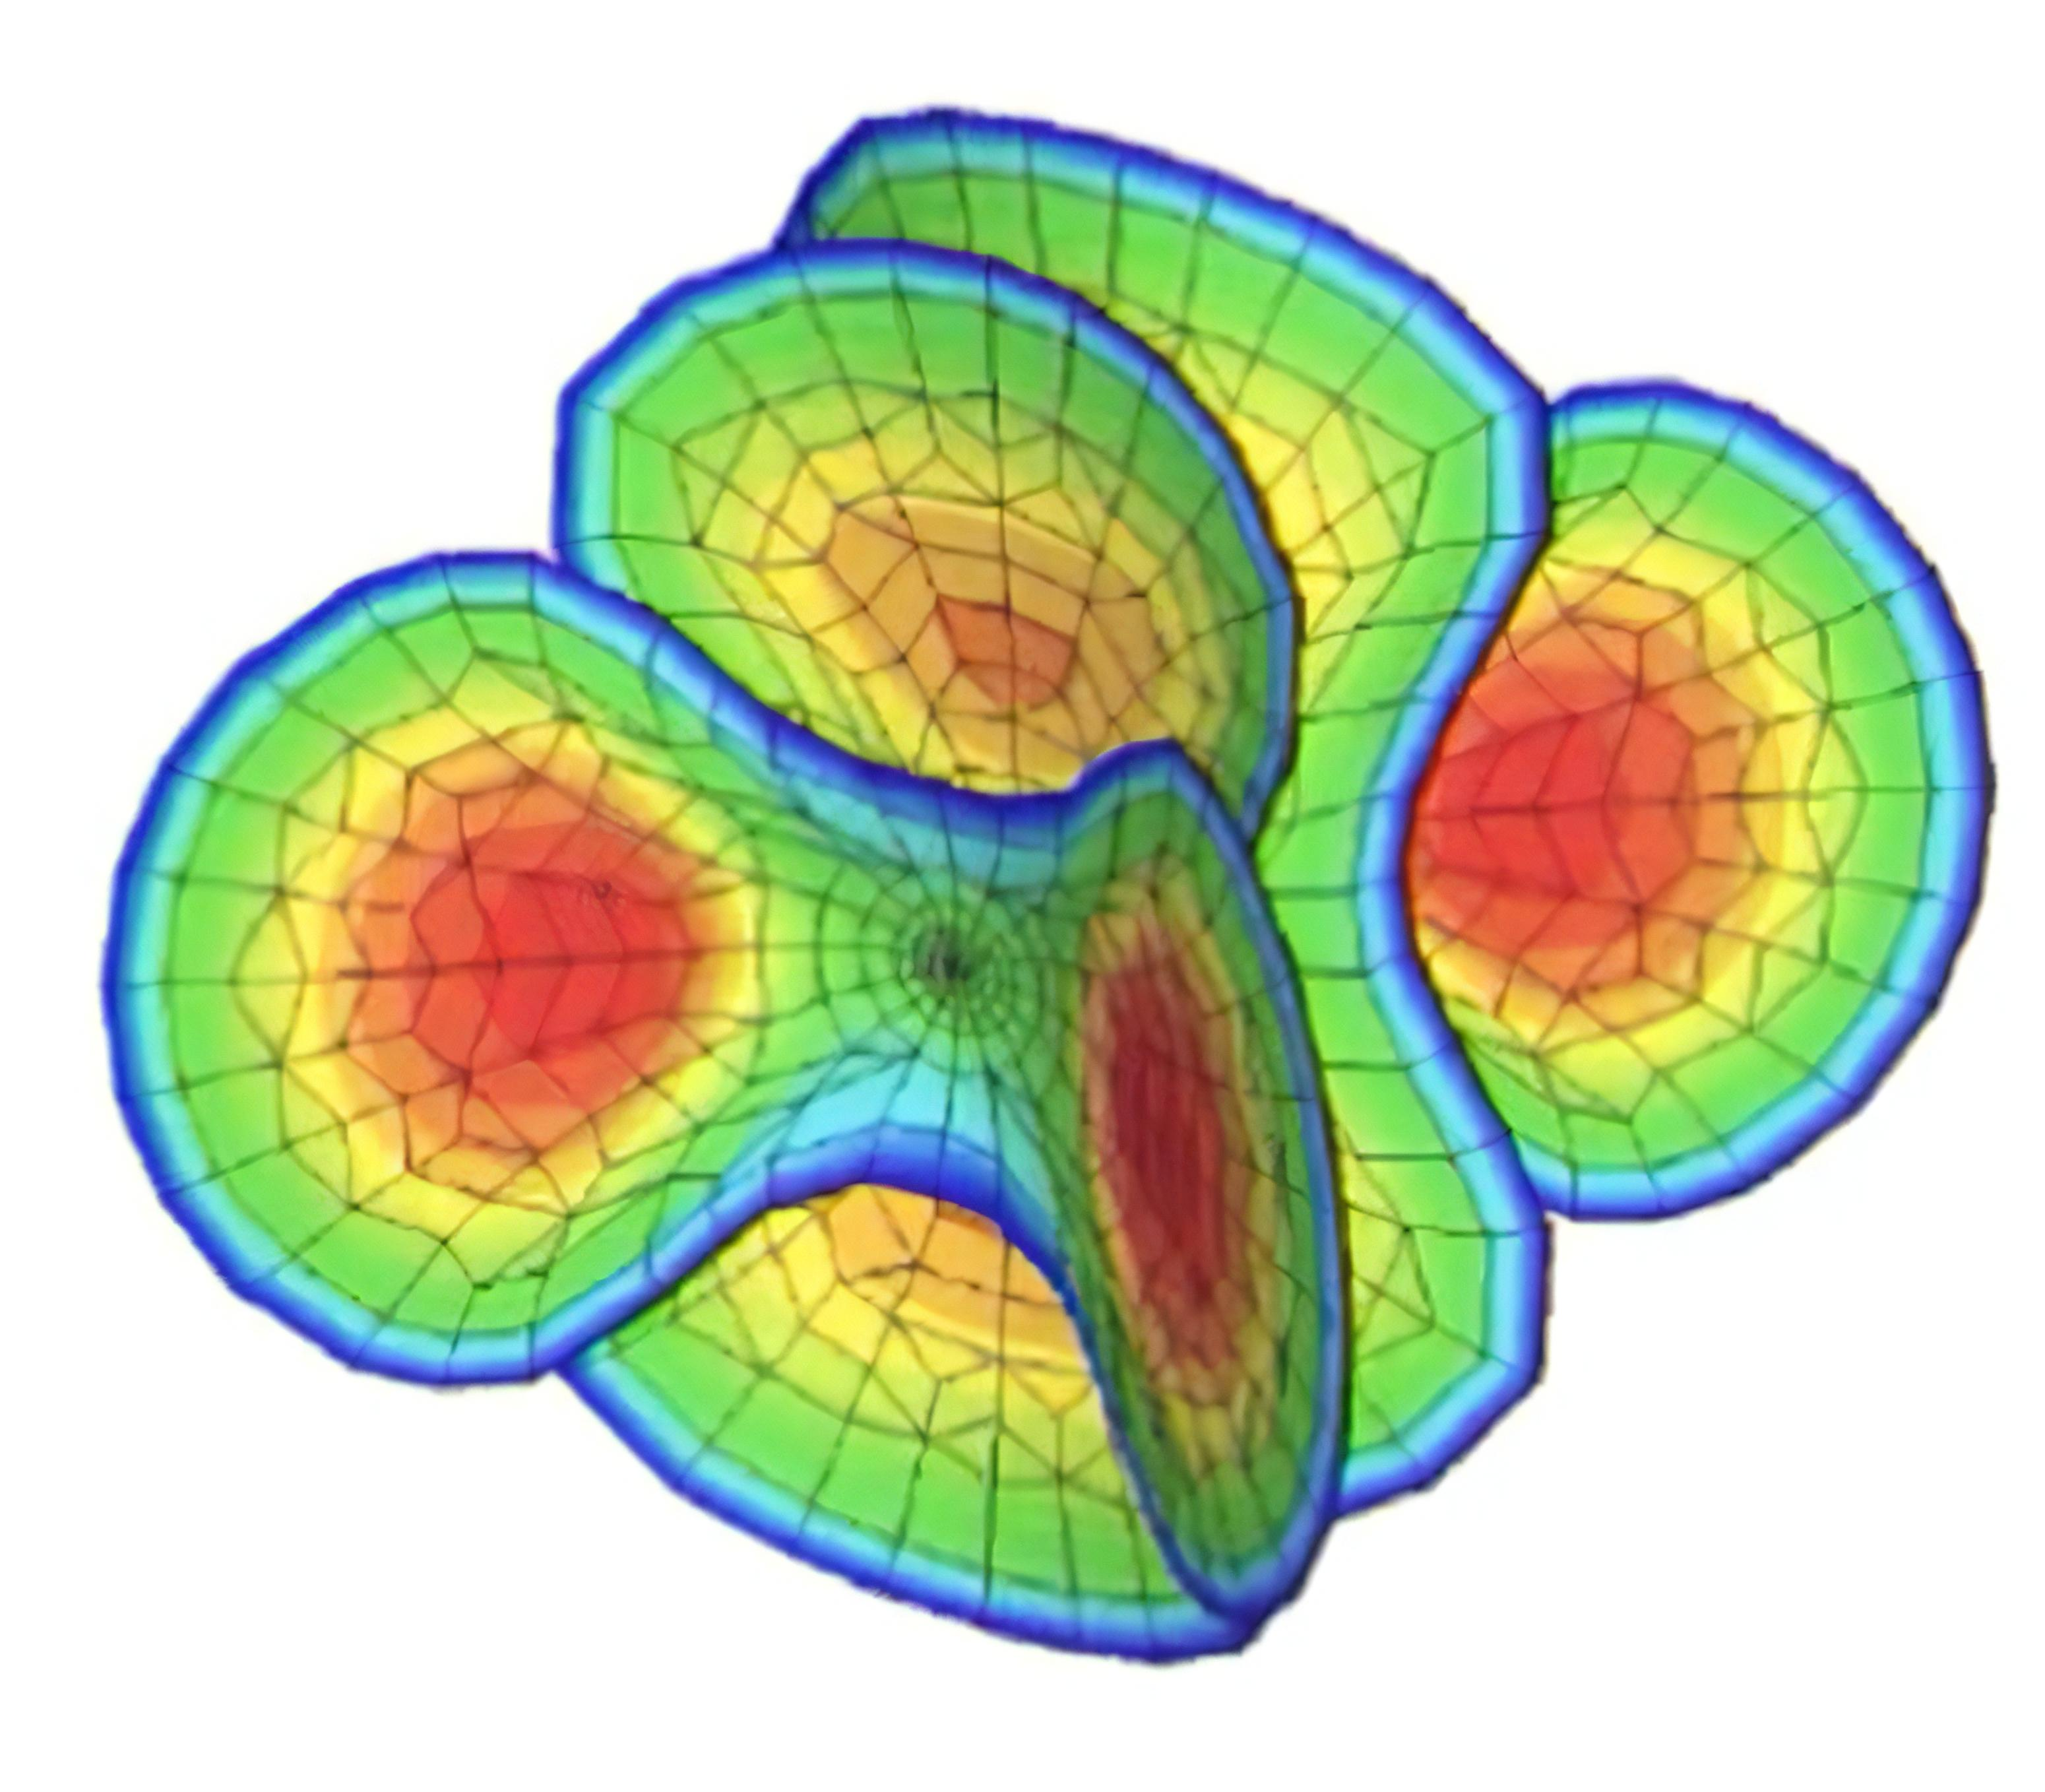
\includegraphics[width=0.6\linewidth]{images/full3D_scheme_better.jpg}}\\ \hline
	Planar3D&Одна трещина, распространяющаяся в плоскости вдоль направления максимальных горизонтальных напряжений; среда однородна по $E$ и $\nu$; законы упругости рассматриваются в рамках линейно-упругой механики разрушения; ньютоновская жидкость с вязкостью $\mu$, отсутствует fluid lag&\hfill\break\makecell[c]{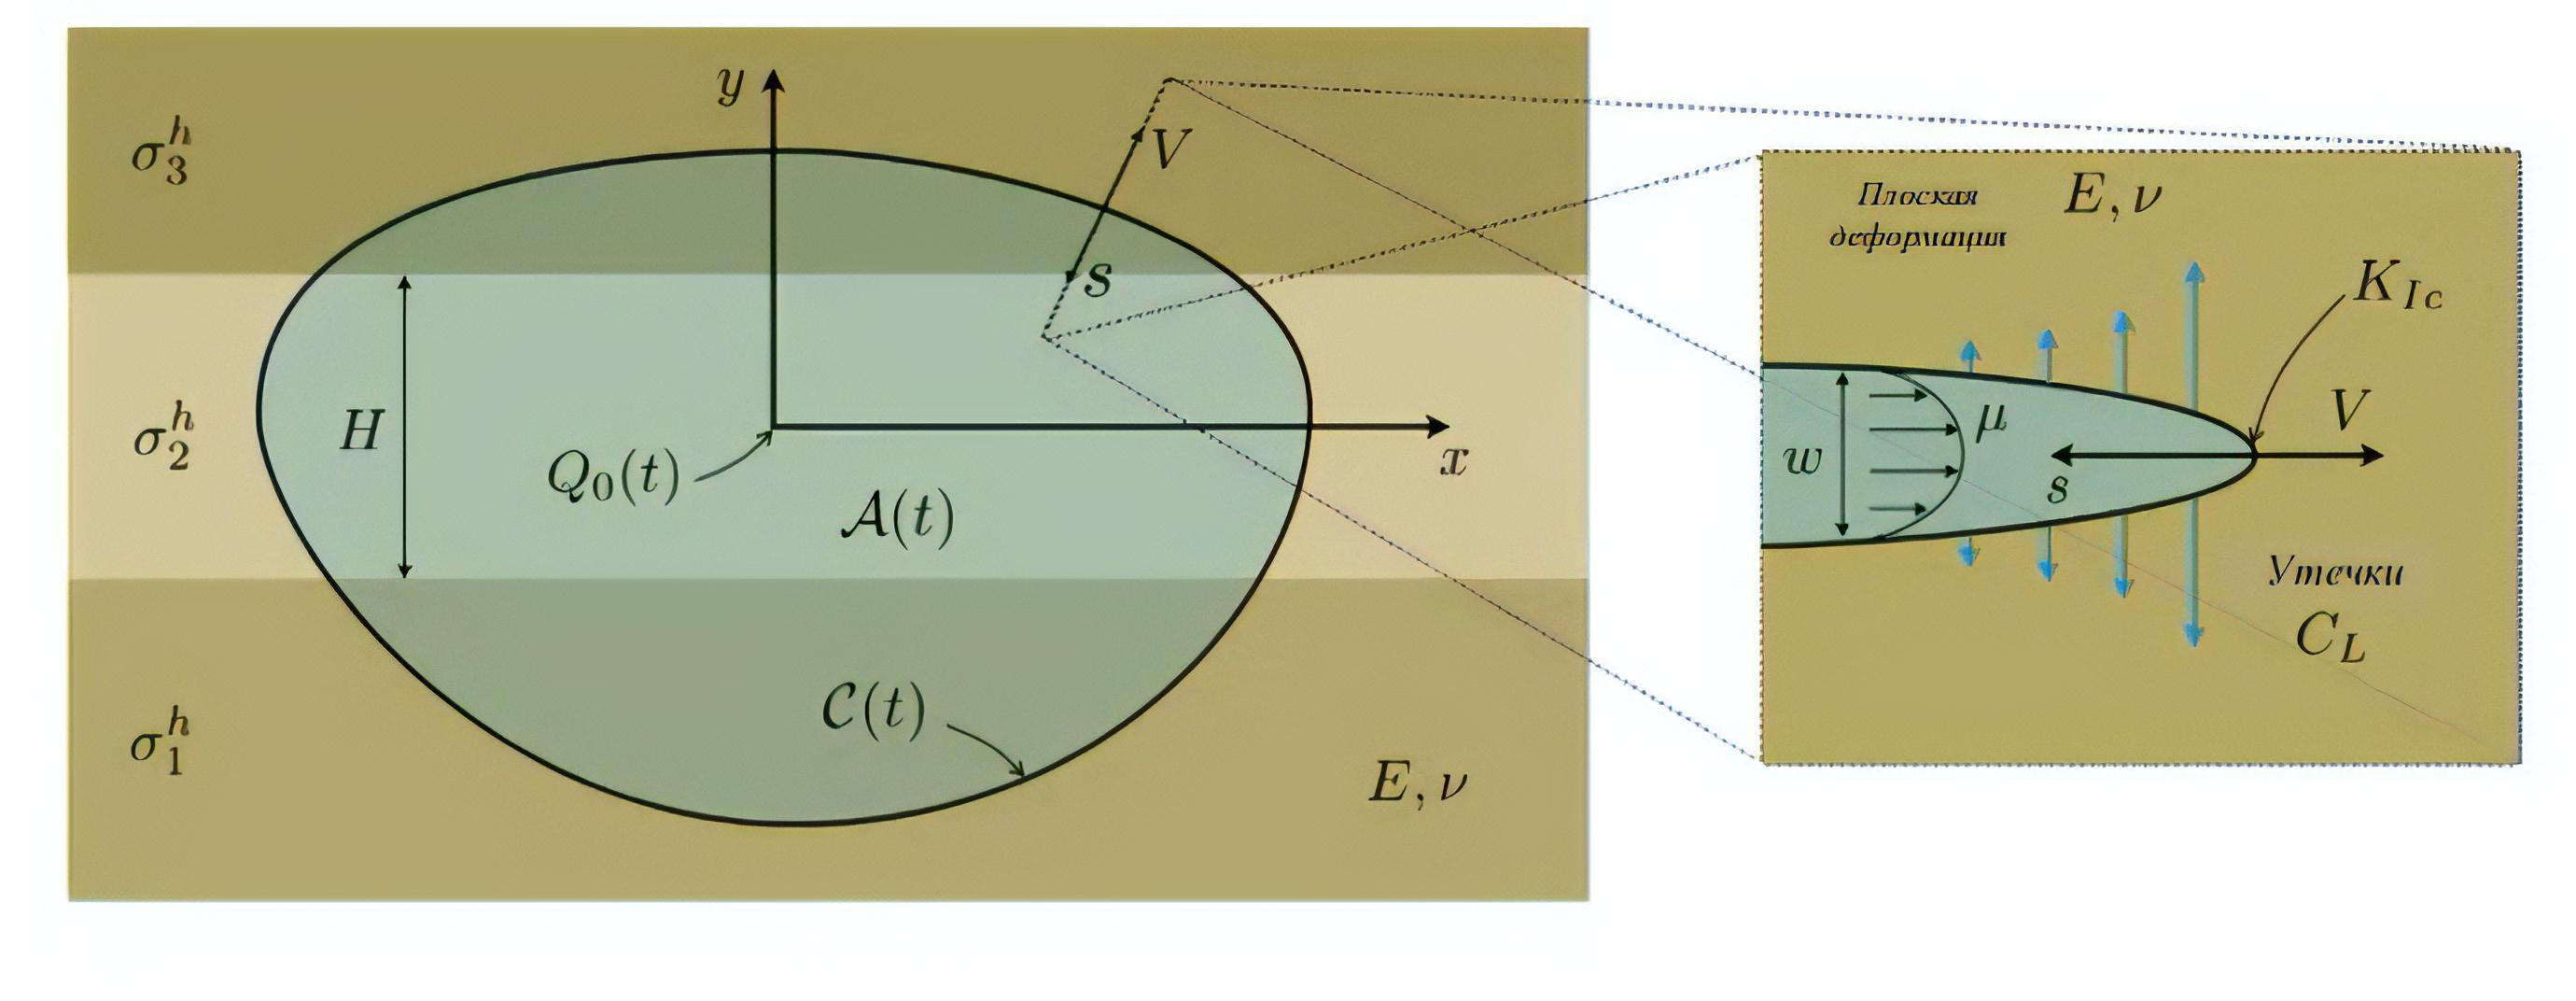
\includegraphics[width=\linewidth]{images/planar3D_scheme_better.jpg}}\\ \hline
	Pseudo3D&Одномерное течение жидкости&\hfill\break\makecell[c]{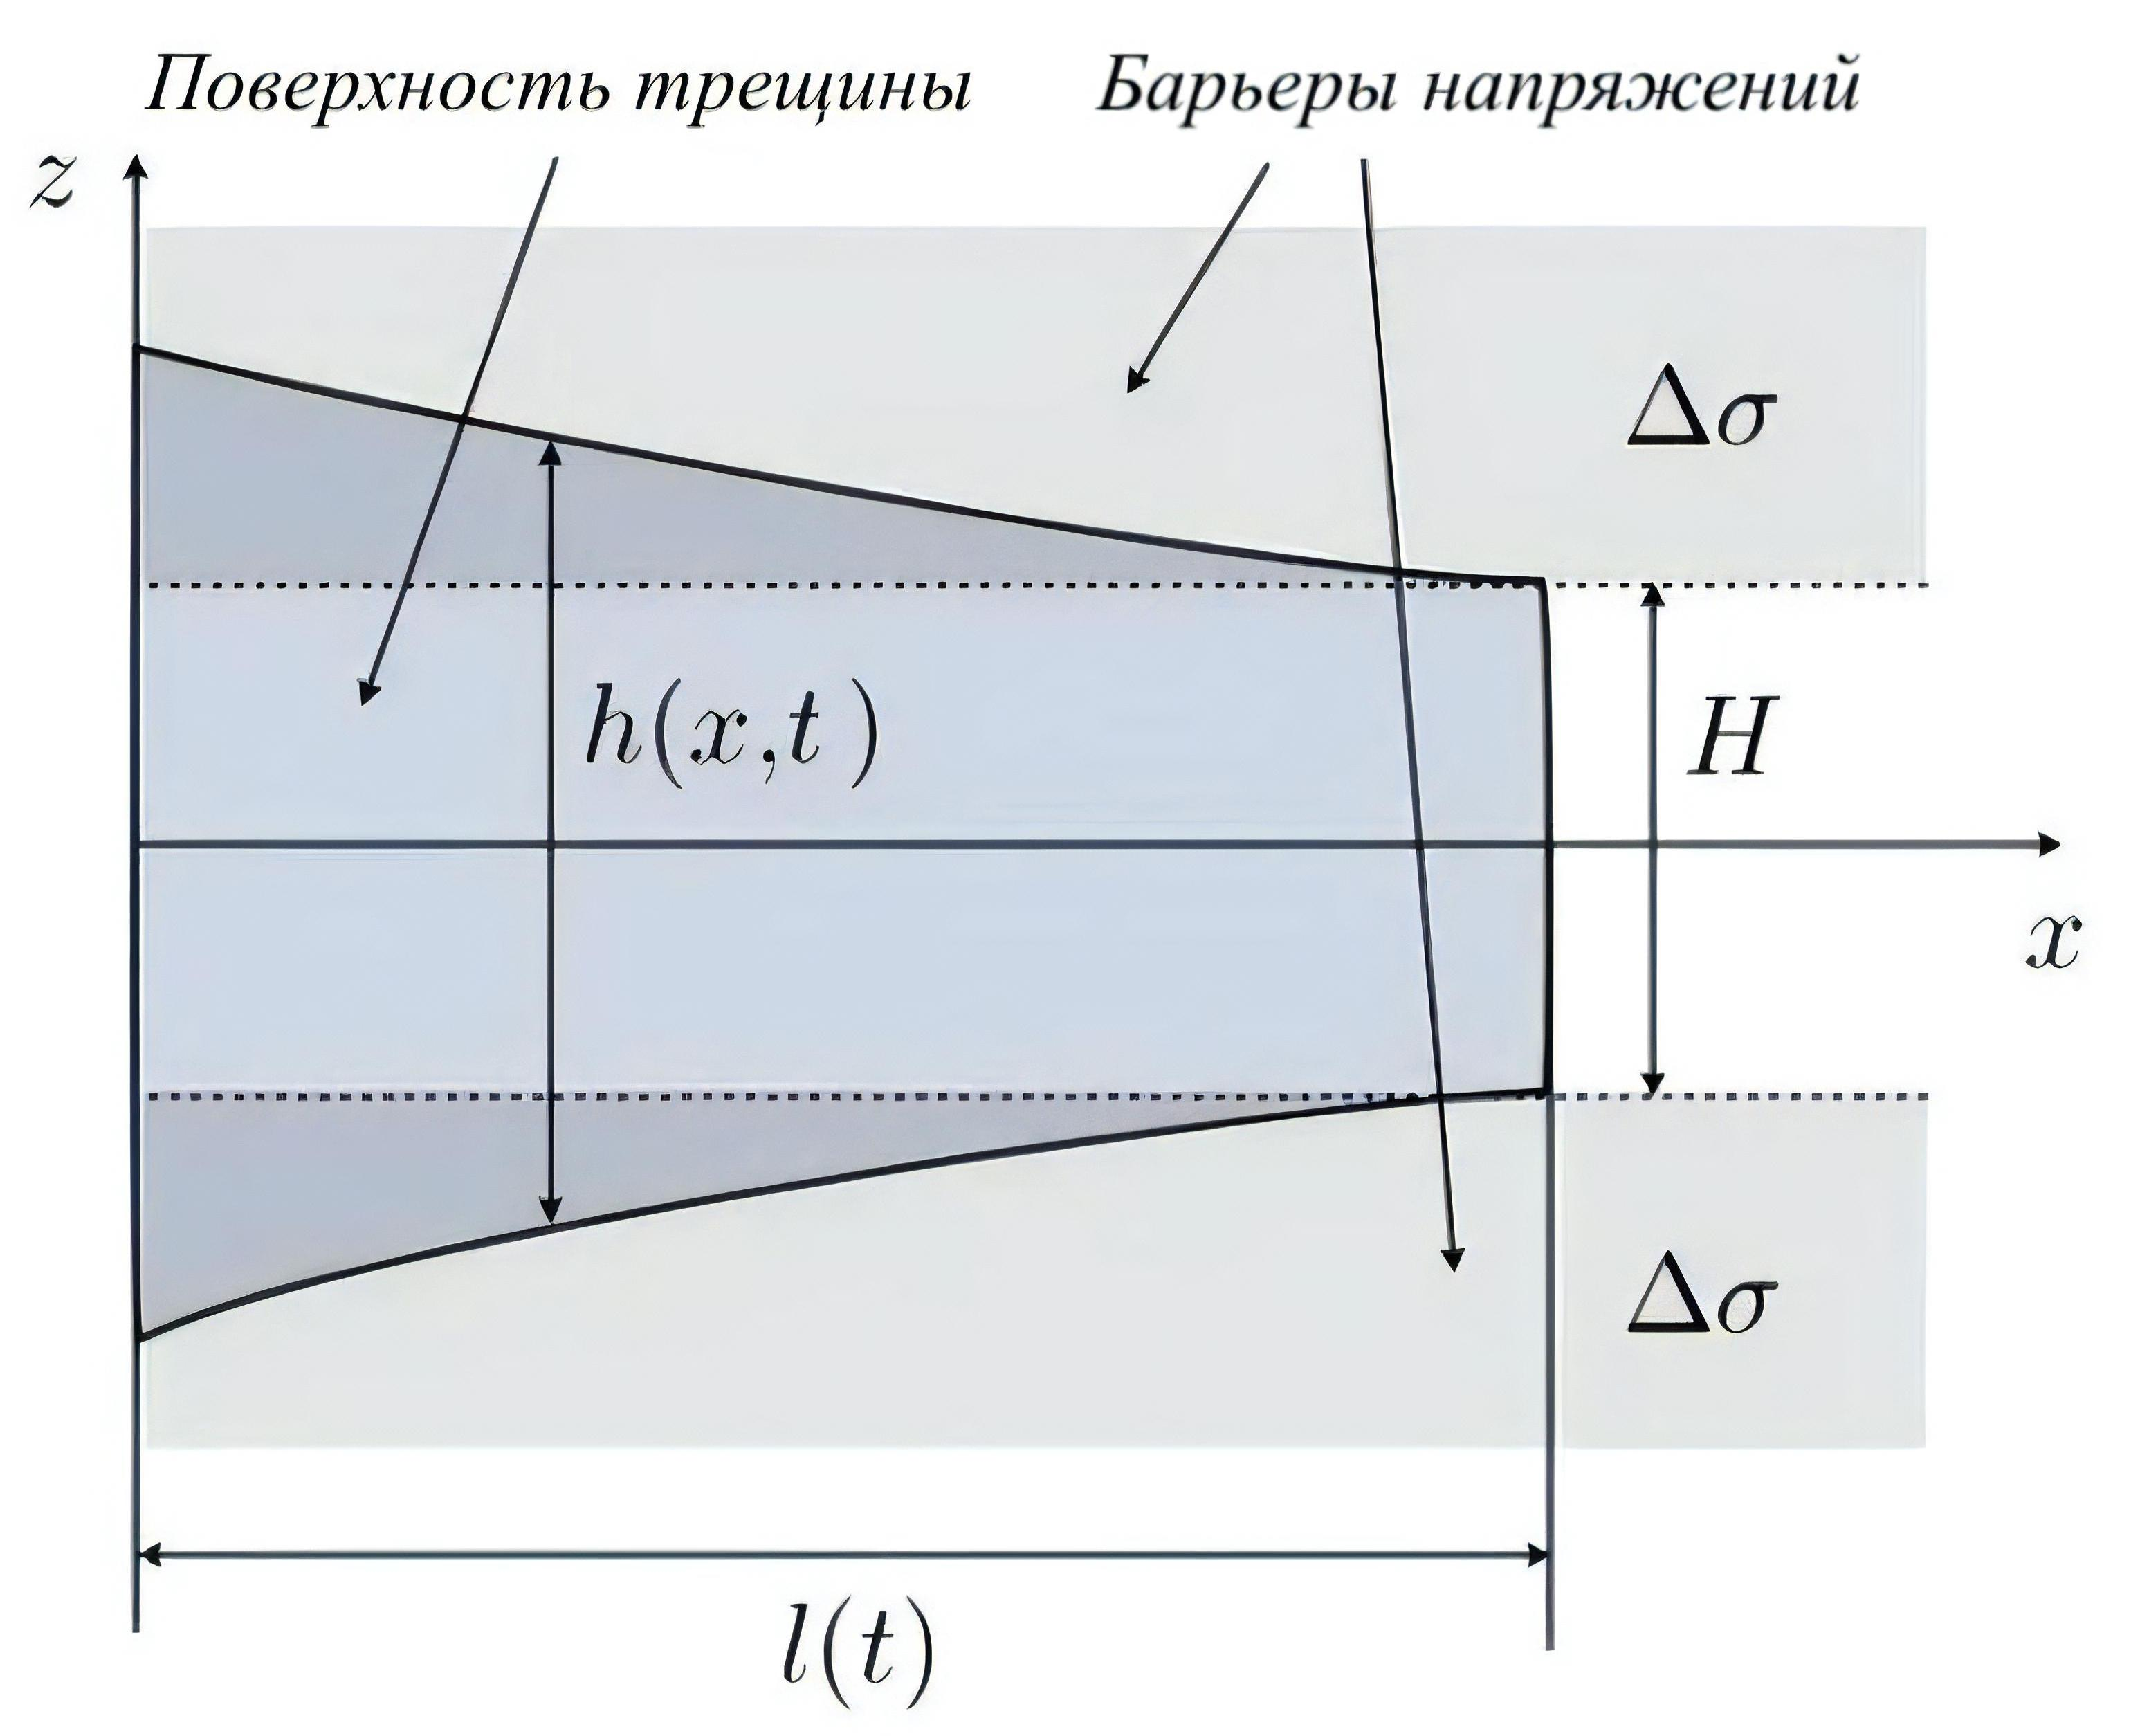
\includegraphics[width=\linewidth]{images/pseudo3D_scheme_better.jpg}}\\ \hline
	Перкинса- Керна- Нордгрена (PKN)&Длина трещины много больше её фиксированной высоты $H$; в каждом вертикальном сечении давление одинаково по сечению (из этого условия следует эллиптичность вертикального сечения трещины)&\hfill\break\makecell[c]{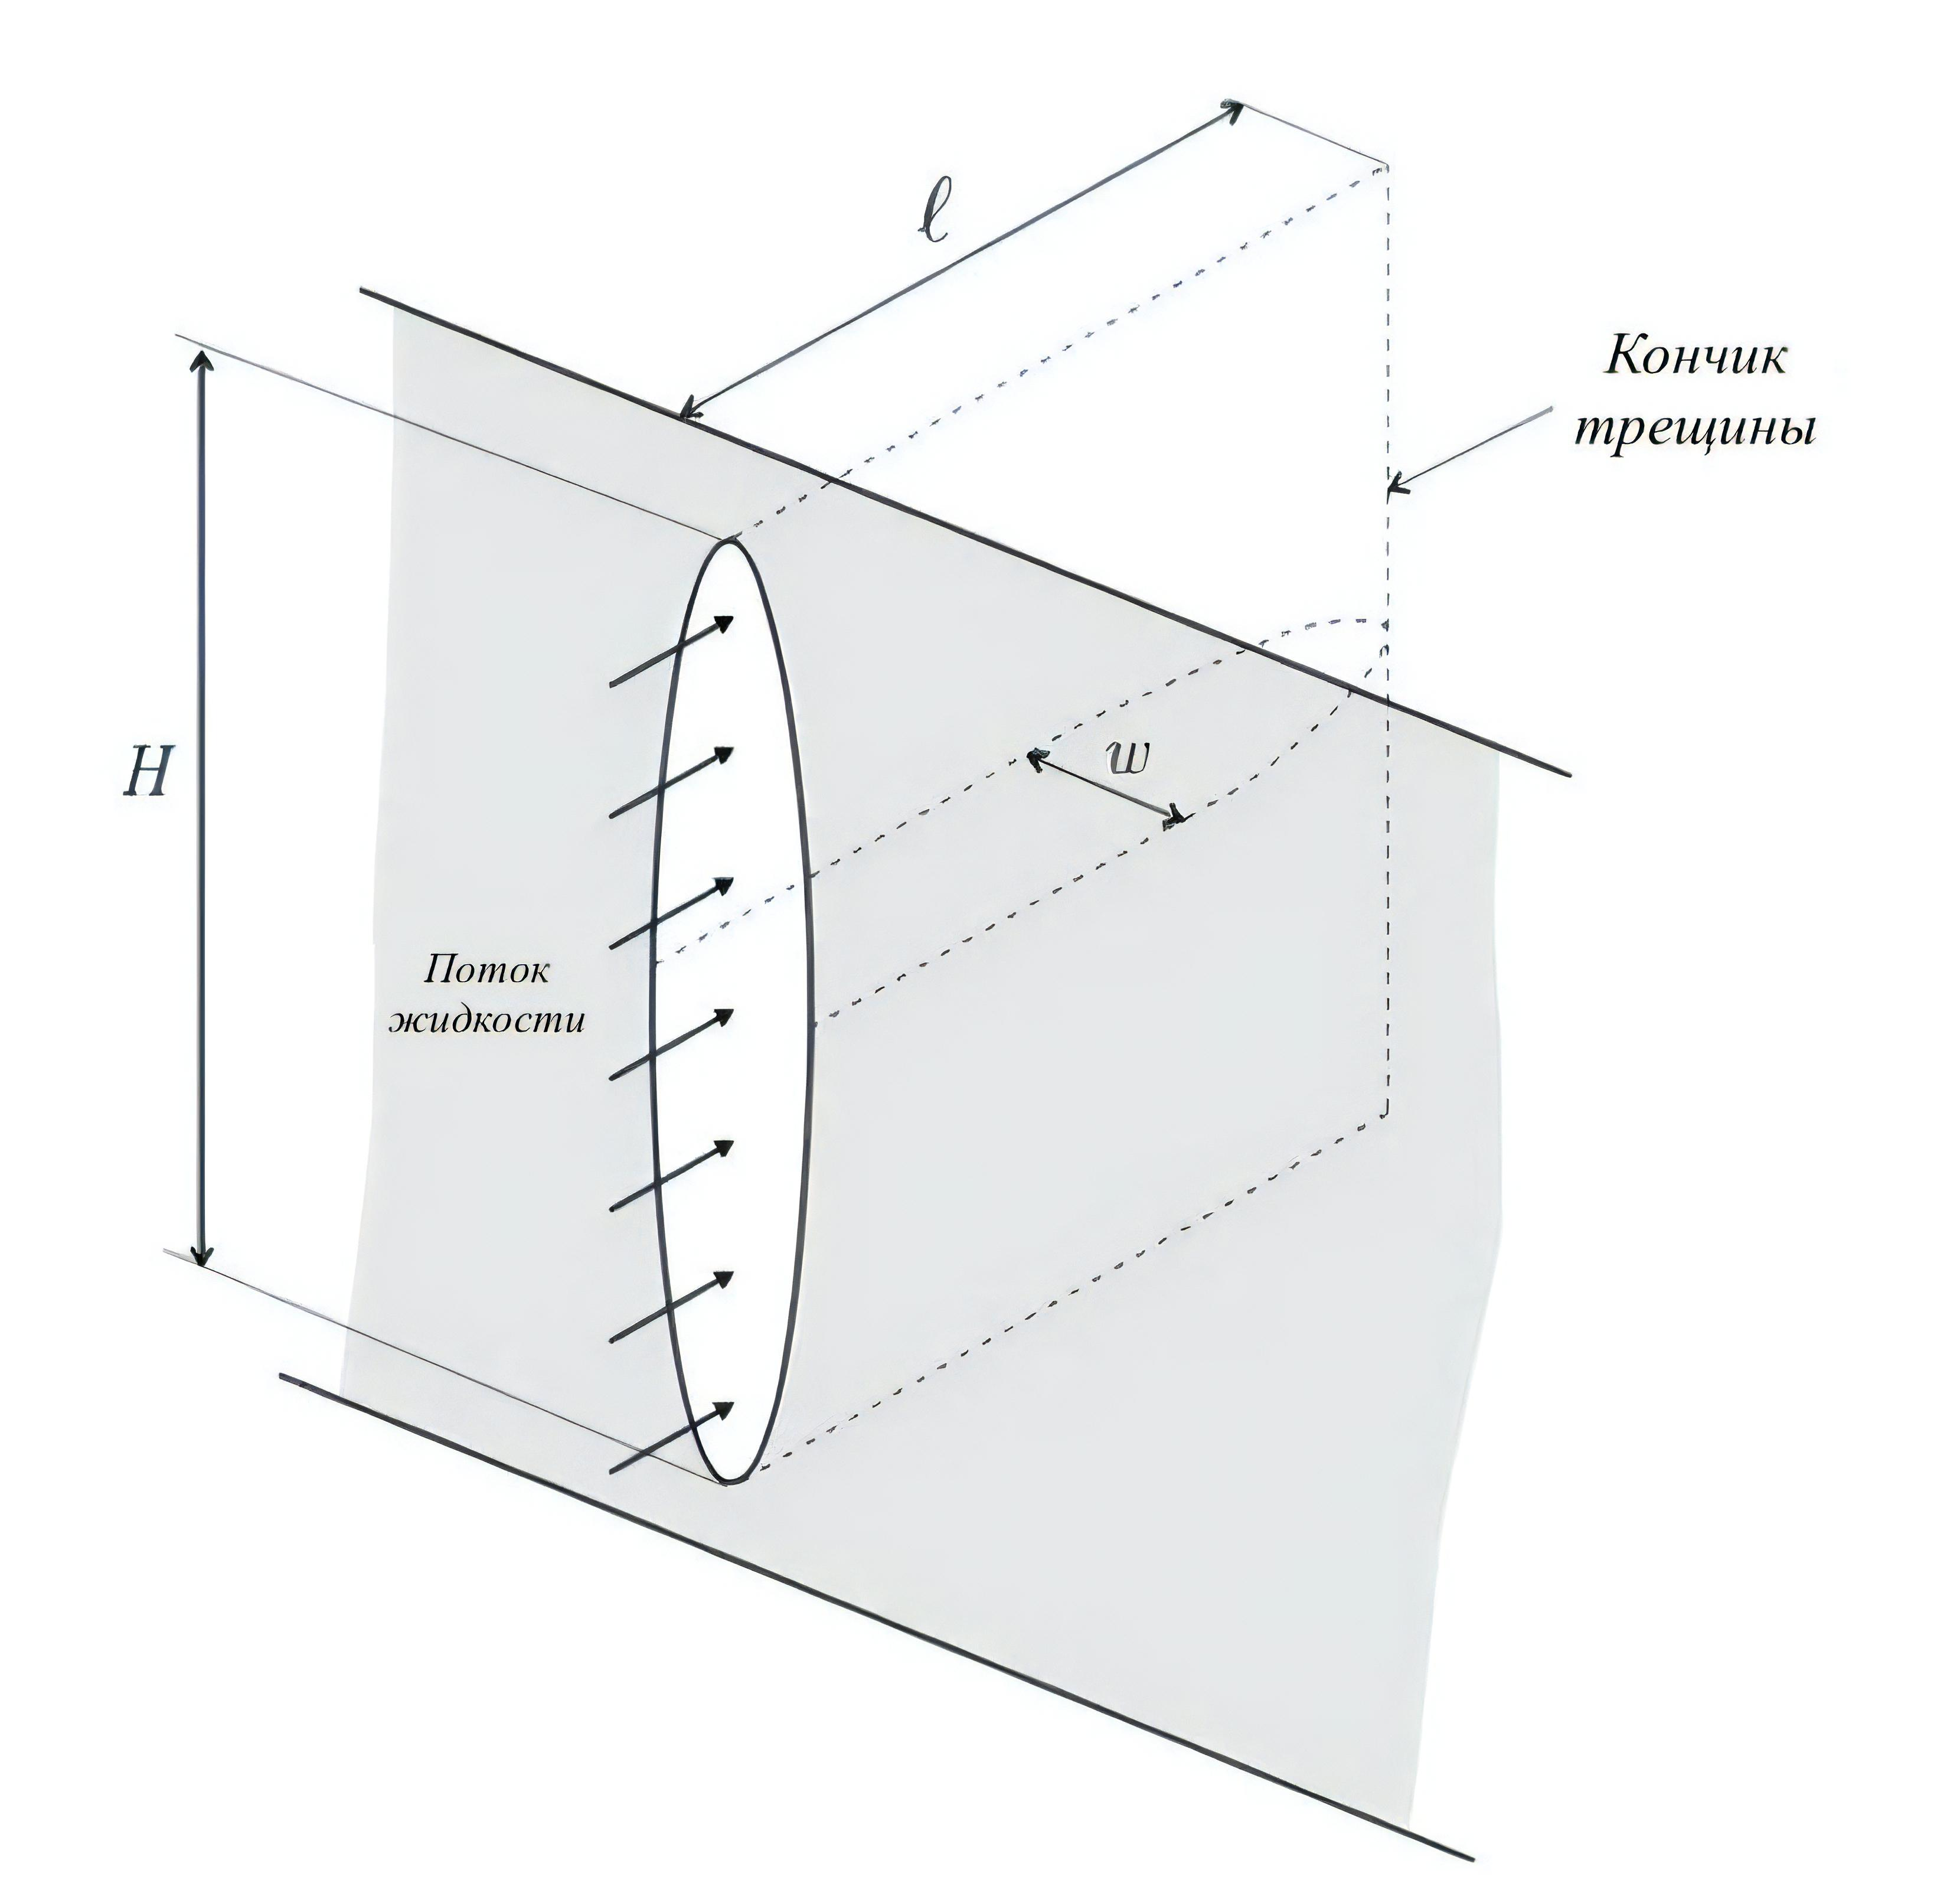
\includegraphics[width=\linewidth]{images/pkn_scheme_better.jpg}}\\ \hline
	Радиальная&Точечный перфорационный интервал; бесконечный по всем направлениям и однородный пласт&\hfill\break\makecell[c]{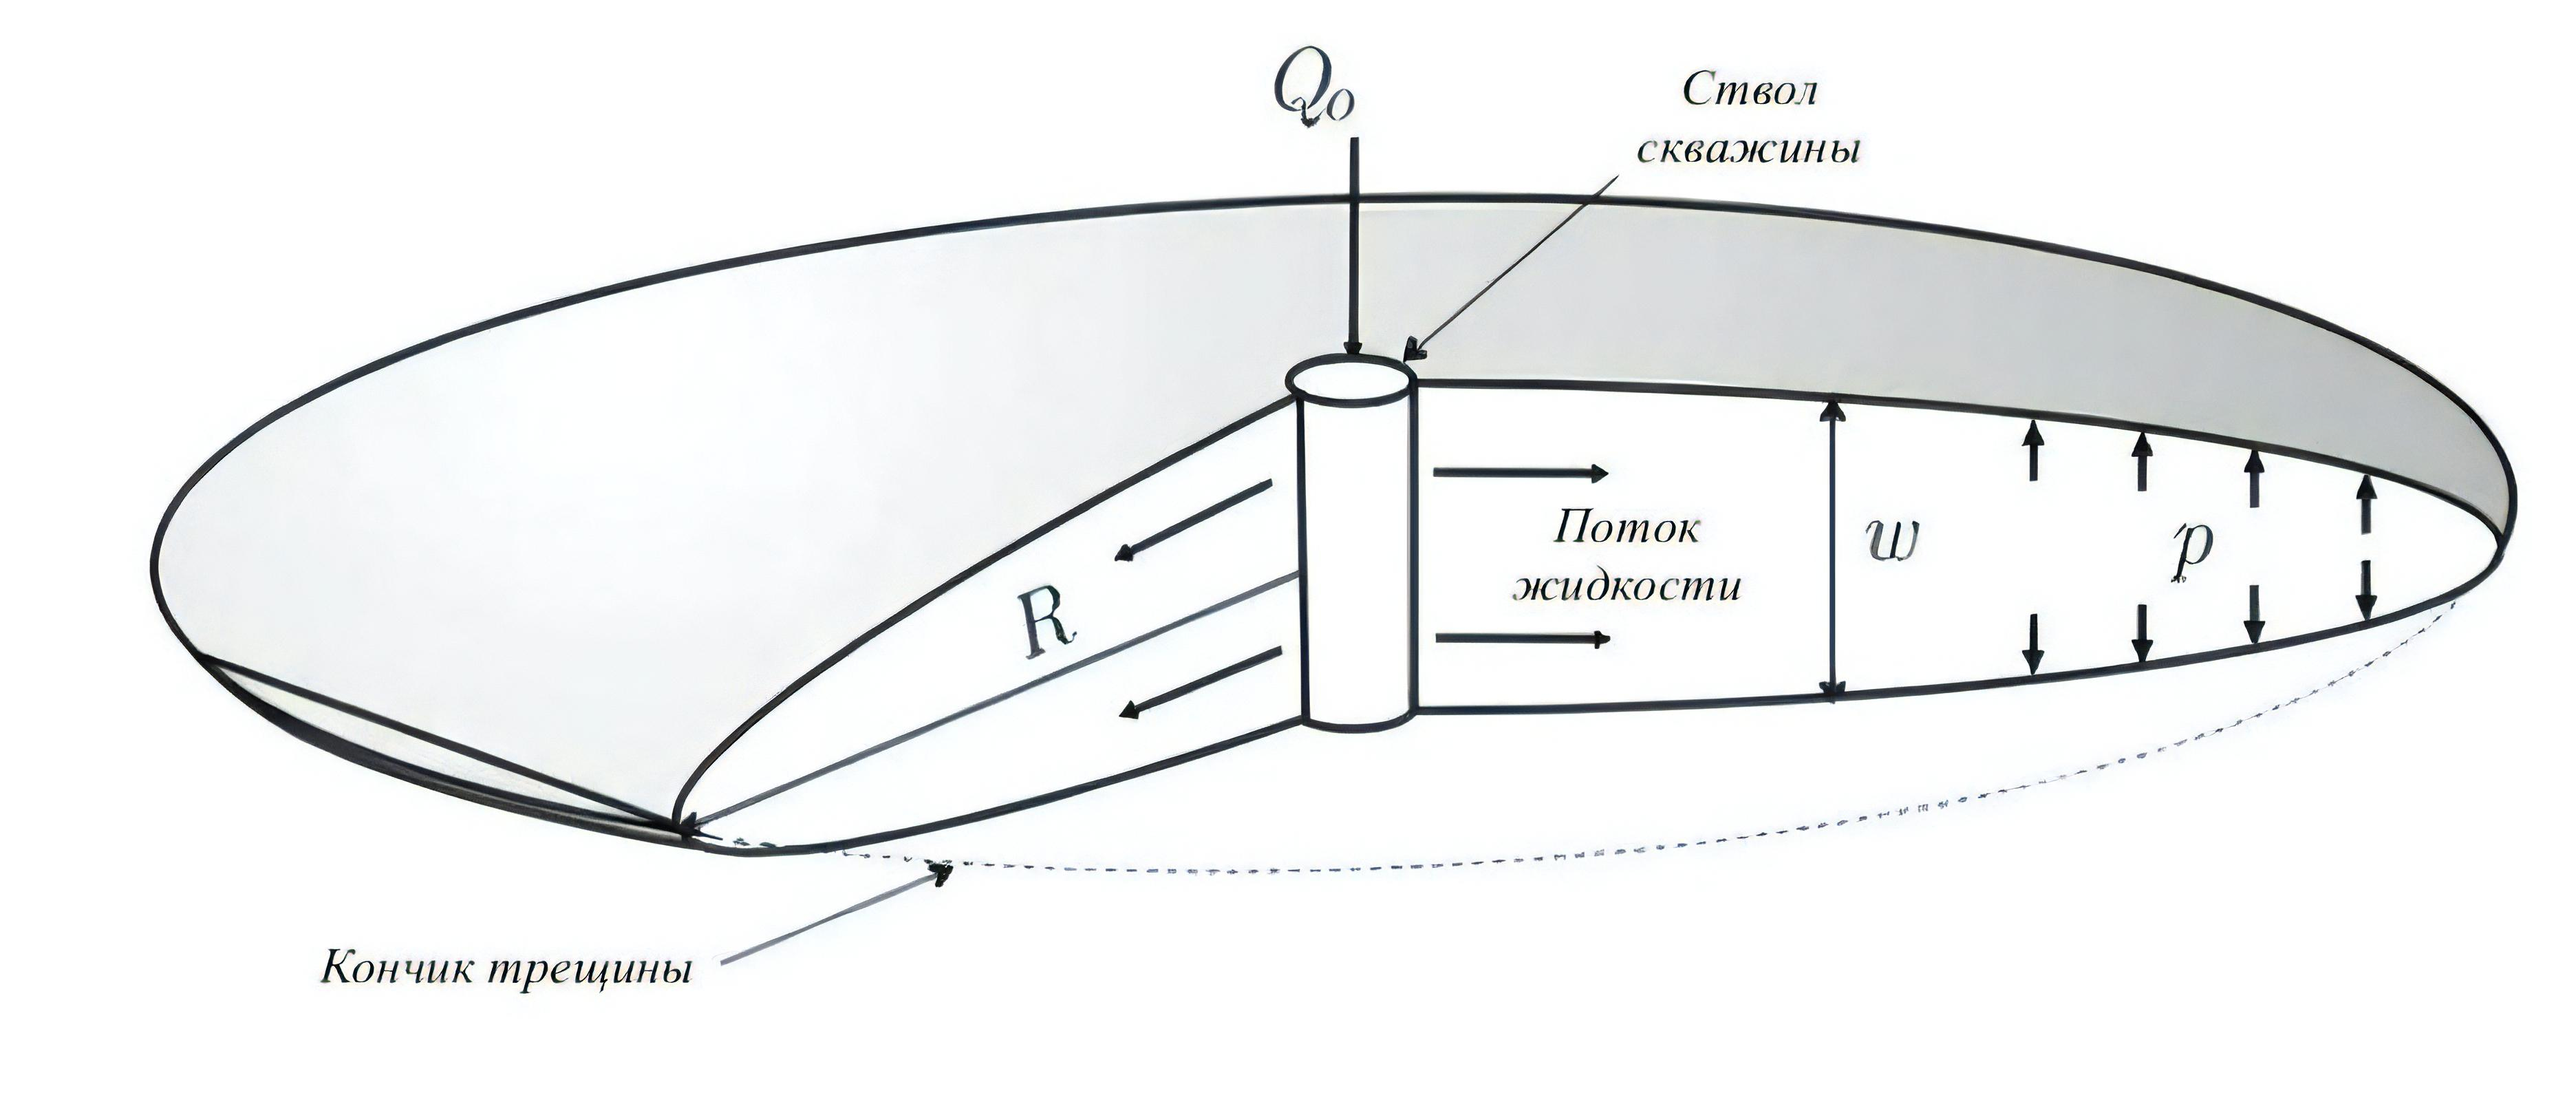
\includegraphics[width=\linewidth]{images/radial_scheme_better.jpg}}\\ \hline
	Христиановича- Желтова- Гиртсма- деКлерка (KGD)&Высота трещины много больше её длины; вертикальное сечение трещины прямоугольно; в горизонтальной плоскости выполняется условие плоской деформации&\hfill\break\makecell[c]{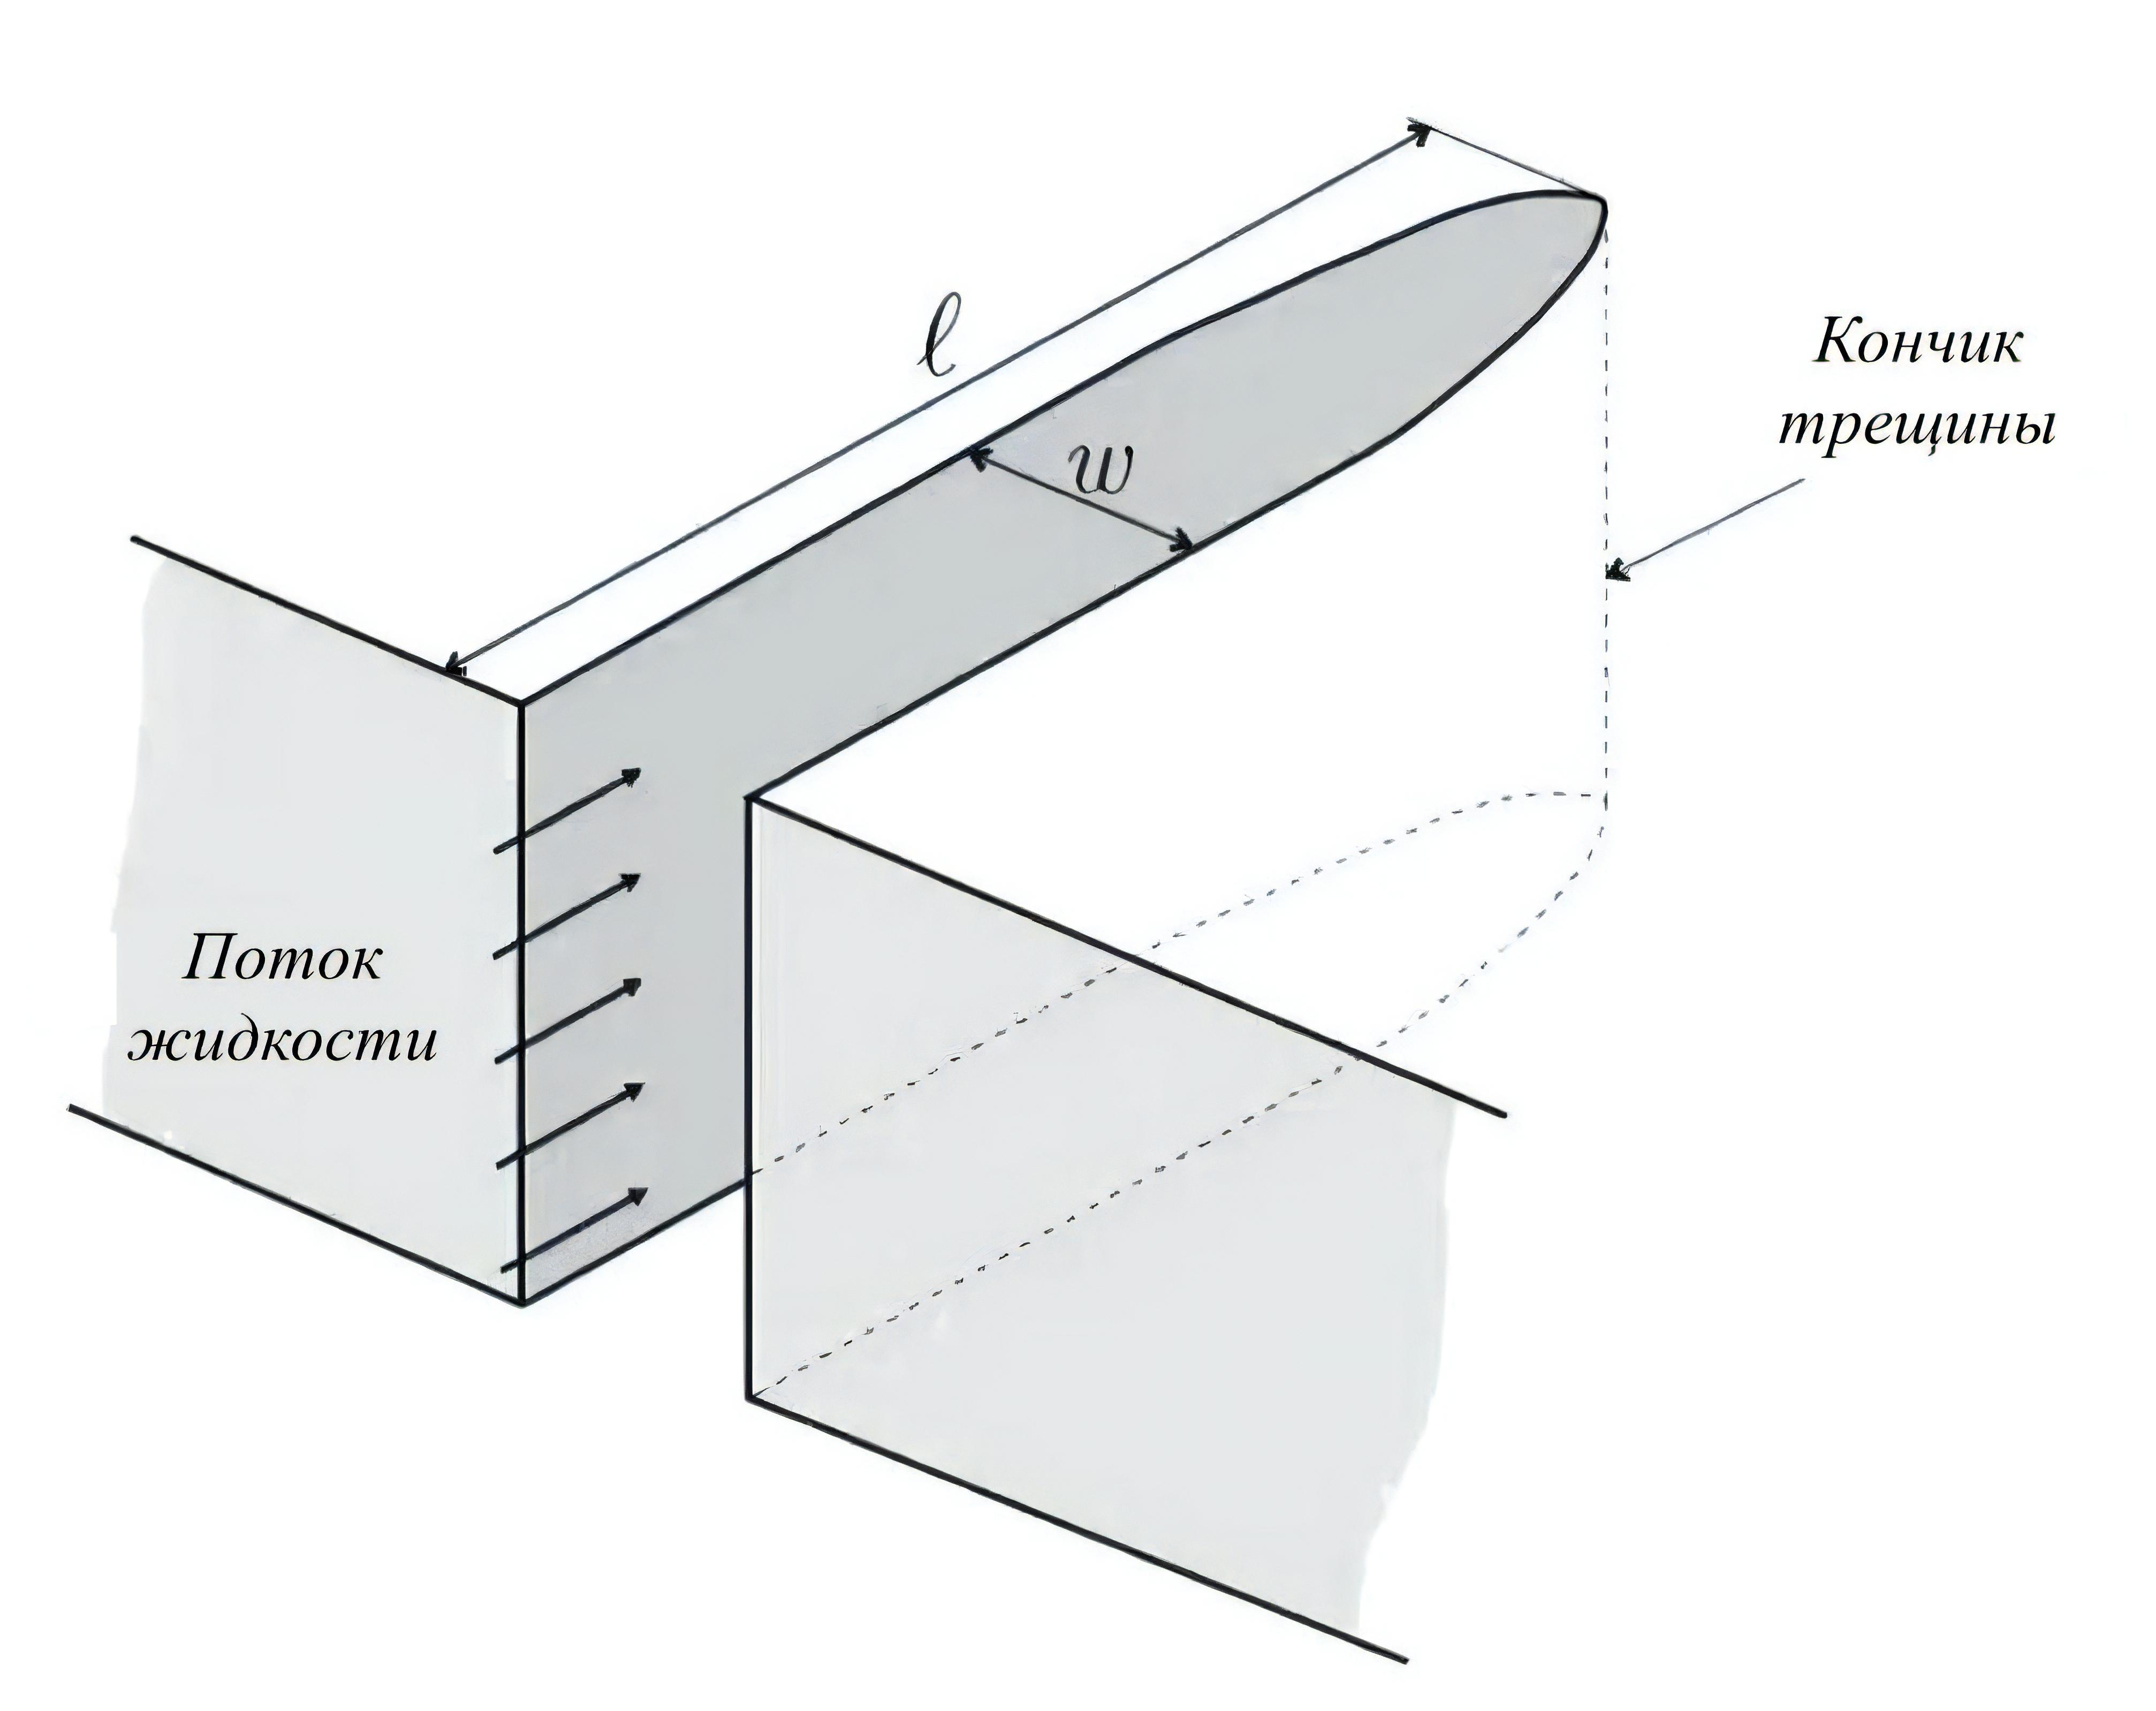
\includegraphics[width=\linewidth]{images/kgd_scheme_better.jpg}}\\ \hline
	
\end{longtable}
\normalsize% возвращаем шрифт к нормальному
\endgroup

Исторически первой С.А.Христиановичем и Ю.П.Желтовым (и независимо от них Гиртсма и деКлерком) в 1955 году была разработана модель KGD, которая хорошо описывает поведение трещины, распространяющейся из протяжённого перфорированного интервала, на ранних временах её распространения.

Также была разработана модель радиальной трещины ГРП, которая реализуется при гидроразрыве относительно мощных однородных пластов из ограниченных (точечных) перфорированных интервалов.

Позже в 1961 году исследователями Перкинсом и Керном была разработана более распространённая модель Перкинса-Керна, которая хорошо описывает поведение трещины, распространяющейся из протяжённого перфорированного интервала, на поздних временах её распространения.
В дальнейшем Нордгреном к модели Перкинса-Керна были добавлены эффекты потери жидкости.

Любая модель трещины гидроразрыва пласта состоит из нескольких основных компонентов:

1) уравнения баланса жидкости с учётом утечек;

2) модели жидкости;

3) уравнения упругости;

4) условия распространения;

5) модели транспорта проппанта.

Далее будут представлены математические модели трещины KGD, радиальной и PKN.

\section{Модель Христиановича-Желтова-Гиртсма-деКлерка}

В первой модели гидроразрыва пласта, разработанной С.А.Христиановичем и Ю.П.Желтовым, рассматривается трещина одной и той же ширины на любой вертикальной координате в пределах фиксированной толщины пласта $h$.
Другими словами, используется допущение о плоской деформации в каждой горизонтальной плоскости (это допущение более приемлемо для коротких трещин, у которых $2x_f<h$, где $x_f$ -- полудлина трещины).
В основе лежит физическая гипотеза, что поверхности трещины свободно скользят по кровле и подошве пласта.

В результате получается трещина прямоугольного вертикального сечения, а ширина трещины рассматривается как функция координаты $x$.

\begin{figure}[H] 
\center
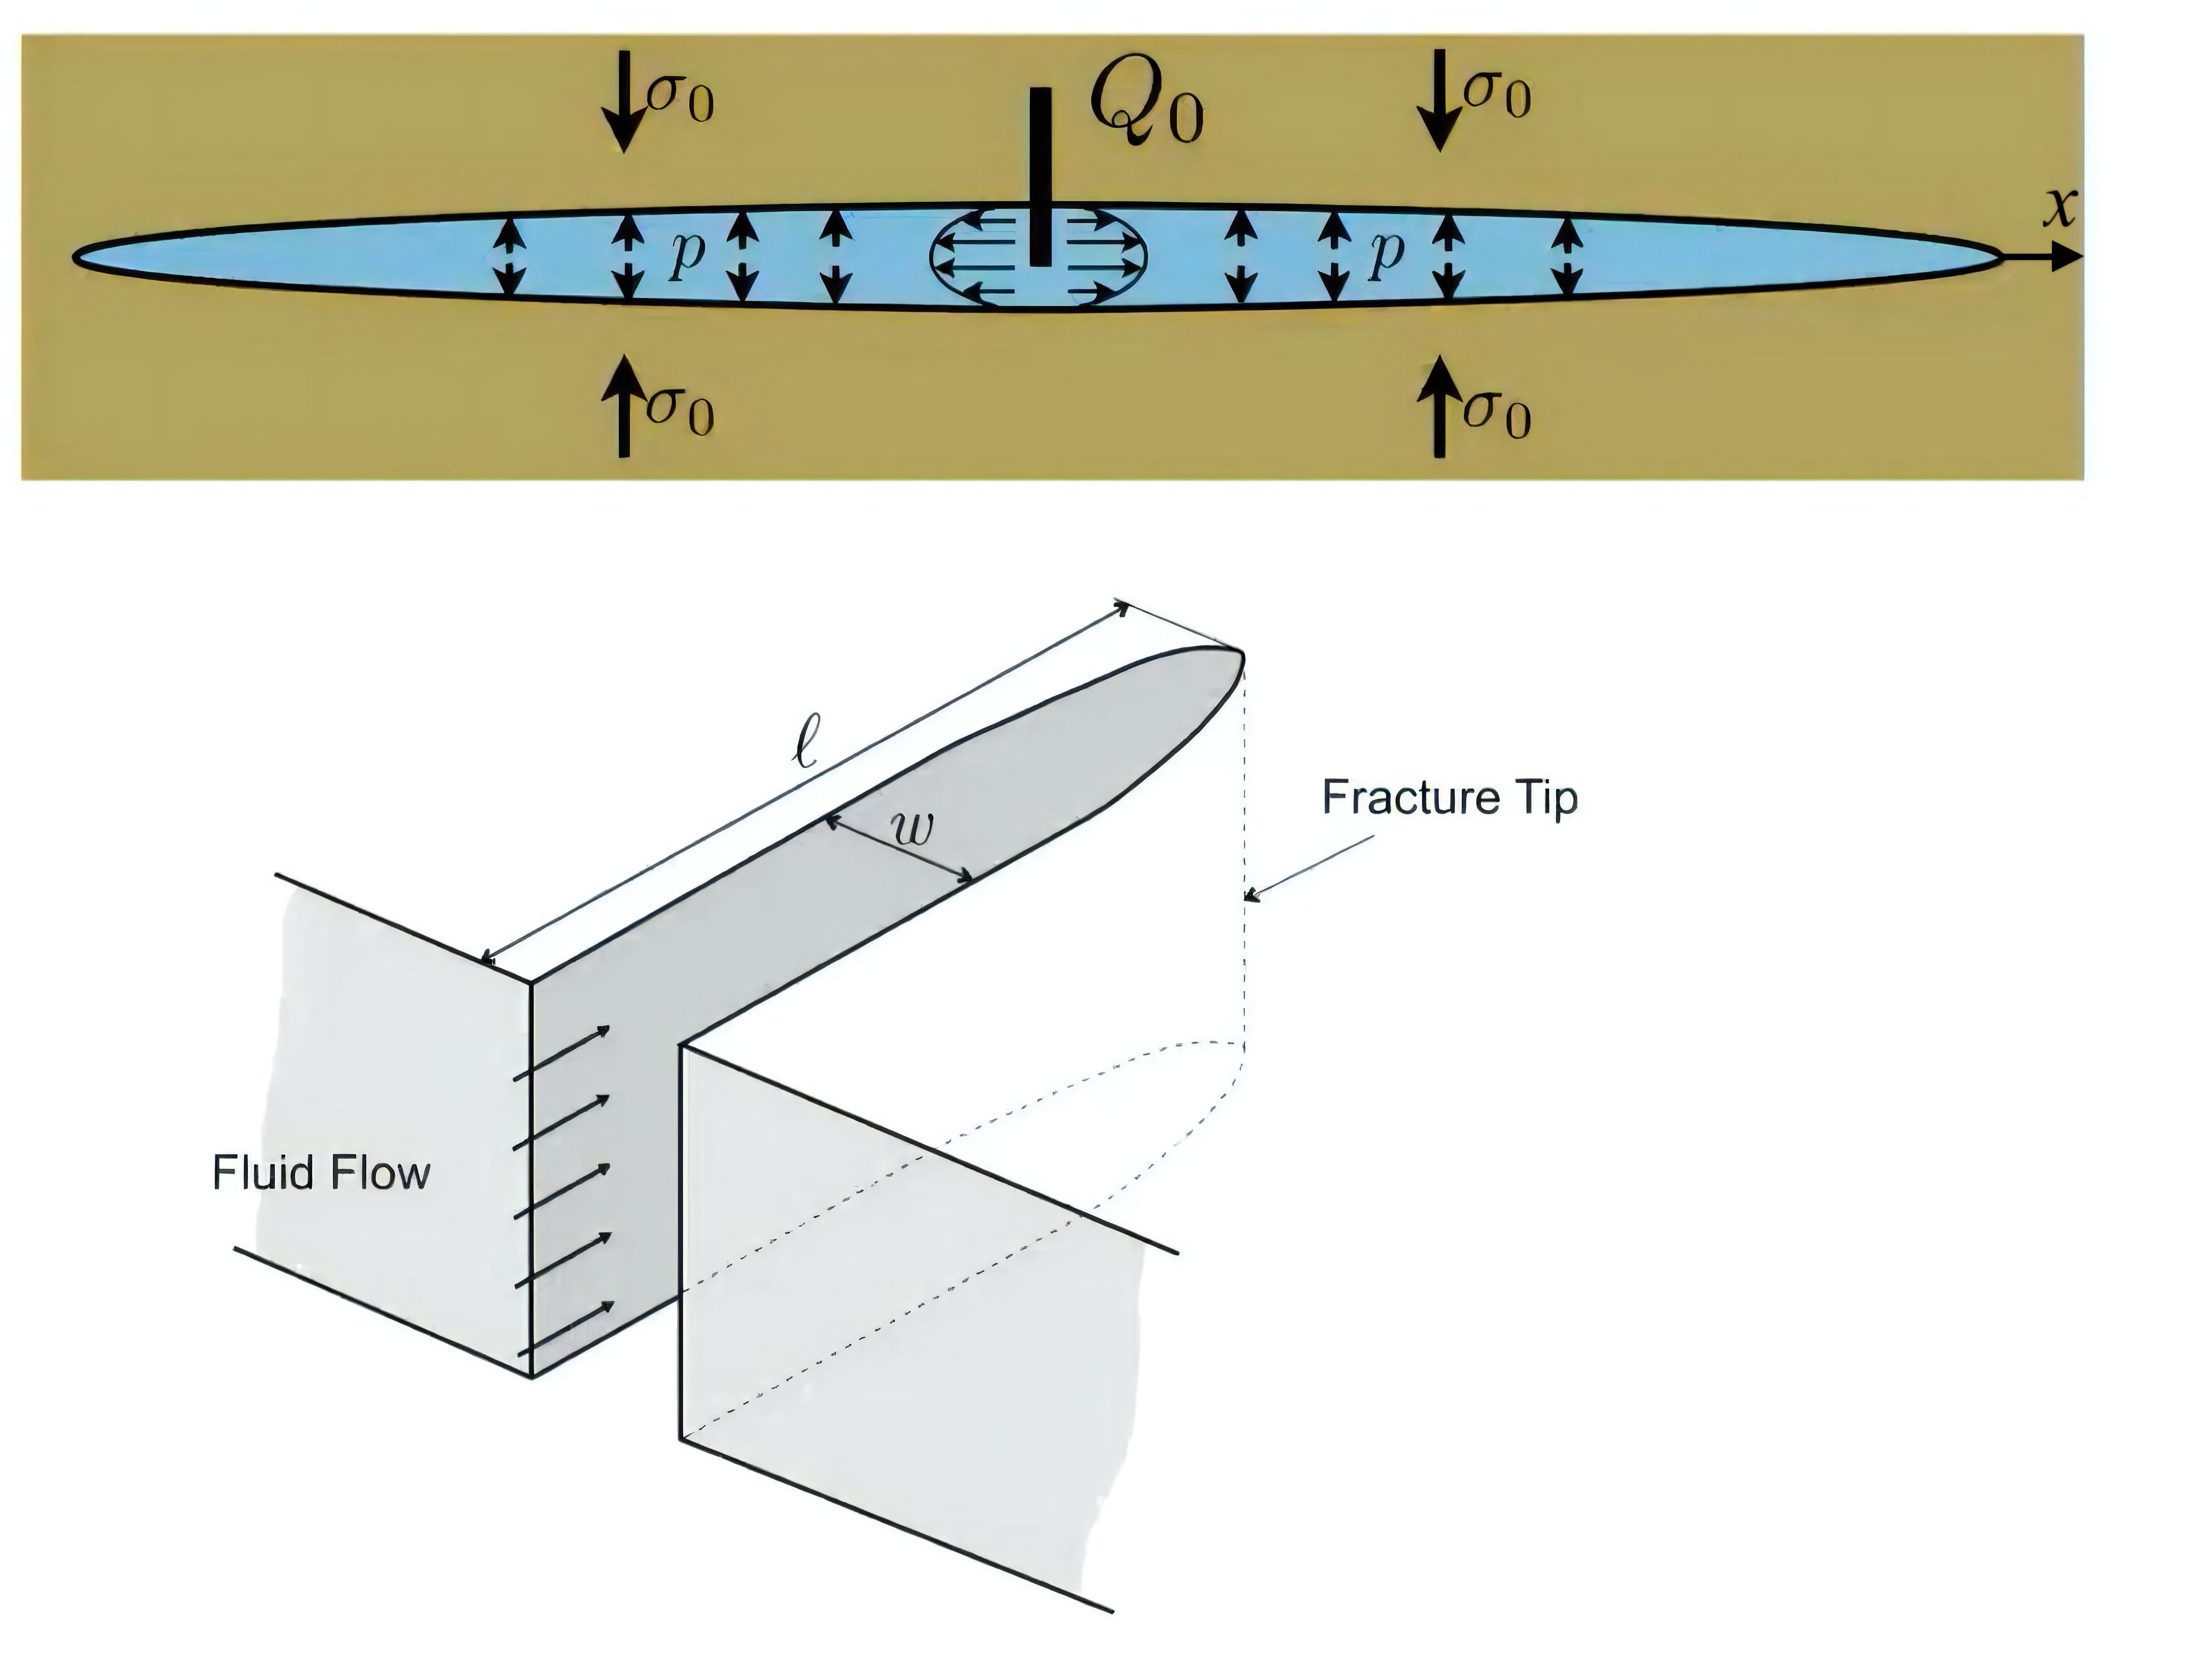
\includegraphics[width=0.7\linewidth]{images/kgd_model_better.jpg}
\caption{Геометрия трещины KGD} 
\label{fig:kgd-model-geometry}  
\end{figure}


Для трещины KGD верно равенство, выражающее закон сохранения объёма жидкости в малом выделенном объёме:
\beq
w(t+dt)dx = w(t)dx+q_x(x)dt-q_x(x+dx)dt-2gdxdt
\eeq
Откуда получаем уравнение баланса жидкости:
\beq
\frac{\partial w}{\partial t}+\frac{\partial q_x}{\partial x}+2g=Q_0(t)\delta(x)
\eeq

Из модели Картера скорость утечек:
\beq
g=\frac{C_l}{\sqrt{t-t_0(x)}}
\eeq

Таким образом, уравнение баланса жидкости с учётом утечек для трещины KGD запишется в следующей форме:
\beq
\frac{\partial w}{\partial t}+\frac{\partial q}{\partial x}+\frac{C'}{\sqrt{t-t_0(x)}}=Q_0(t)\delta(x),
\eeq
где $C'=2C_l$.

В модели трещины KGD рассматривается одномерное течение жидкости вдоль трещины, то есть имеется только одна компонента вектора скорости, которая изменяется при движении:
\beq
v=v_x(y)
\eeq
Из уравнения Навье-Стокса:
\beq
\frac{\partial p}{\partial x}=\frac{\partial\tau}{\partial y}
\eeq
Для ньютоновской жидкости:
\beq
\tau = \mu\frac{\partial v}{\partial y}
\eeq
Дополнительно ставим условие неприлипания на границе:
\beq
v|_{y=\pm w/2}=0
\eeq
Общее решение:
\beq
v=\frac{\partial p}{\partial x}\frac{y^2}{2}+Ay+B
\eeq
Решение после учёта граничных условий:
\beq
v=-\frac{\partial p}{\partial x}\frac{w^2-4y^2}{8\mu}
\eeq
Суммарный поток (расход):
\beq
q=\int\limits_{-w/2}^{w/2}v(y)dy=-\frac{w^3}{12\mu}\frac{\partial p}{\partial x}
\eeq
Уравнение упругости для трещины KGD запишется в следующей форме:
\beq
p(x,t)=\sigma_0-\frac{E'}{4\pi}\int\limits_{-l}^{l}{\frac{w(s)ds}{(x-s)^2}},
\eeq
где $E'=\dfrac{E}{1-\nu^2}$.\newline\ \newline
Условие распространения трещины KGD можно представить в виде:
\beq
\lim_{x\to l}\frac{w}{(l-x)^{1/2}}=
\begin{cases}
\dfrac{K'}{E'},\text{ если }v>0\\[15pt]
\dfrac{K_I'}{E'},\text{ если }v=0
\end{cases}
\eeq

Таким образом, система уравнений модели трещины KGD запишется в следующем виде:
\beq
\begin{cases}
\dfrac{\partial w}{\partial t}+\dfrac{\partial q}{\partial x}+\dfrac{C'}{\sqrt{t-t_0(x)}}=Q_0(t)\delta(x),\\[15pt]
q=-\dfrac{w^3}{\mu'}\dfrac{\partial p}{\partial x},\\[5pt]
p(x,t)=\sigma_0-\dfrac{E'}{4\pi}\displaystyle\int\limits_{-l}^{l}\dfrac{w(s)ds}{(x-s)^2},\\[20pt]
\displaystyle\lim_{x\to l}\dfrac{w}{(l-x)^{1/2}}=\dfrac{K'}{E'},
\end{cases}
\eeq
где $C'=2C_l$, $\,\,\,\mu'=12\mu$, $\,\,\,E'=\dfrac{E}{1-\nu^2}$, $\,\,\,K'=\dfrac{8K_{Ic}}{\sqrt{2\pi}}$.
\\

Приближённые решения для модели Христиановича-Желтова-Гиртсма-
деКлерка представлены в работе \cite{dontsov1}.

\section{Модель радиальной трещины ГРП}

\begin{figure}[H] 
\center
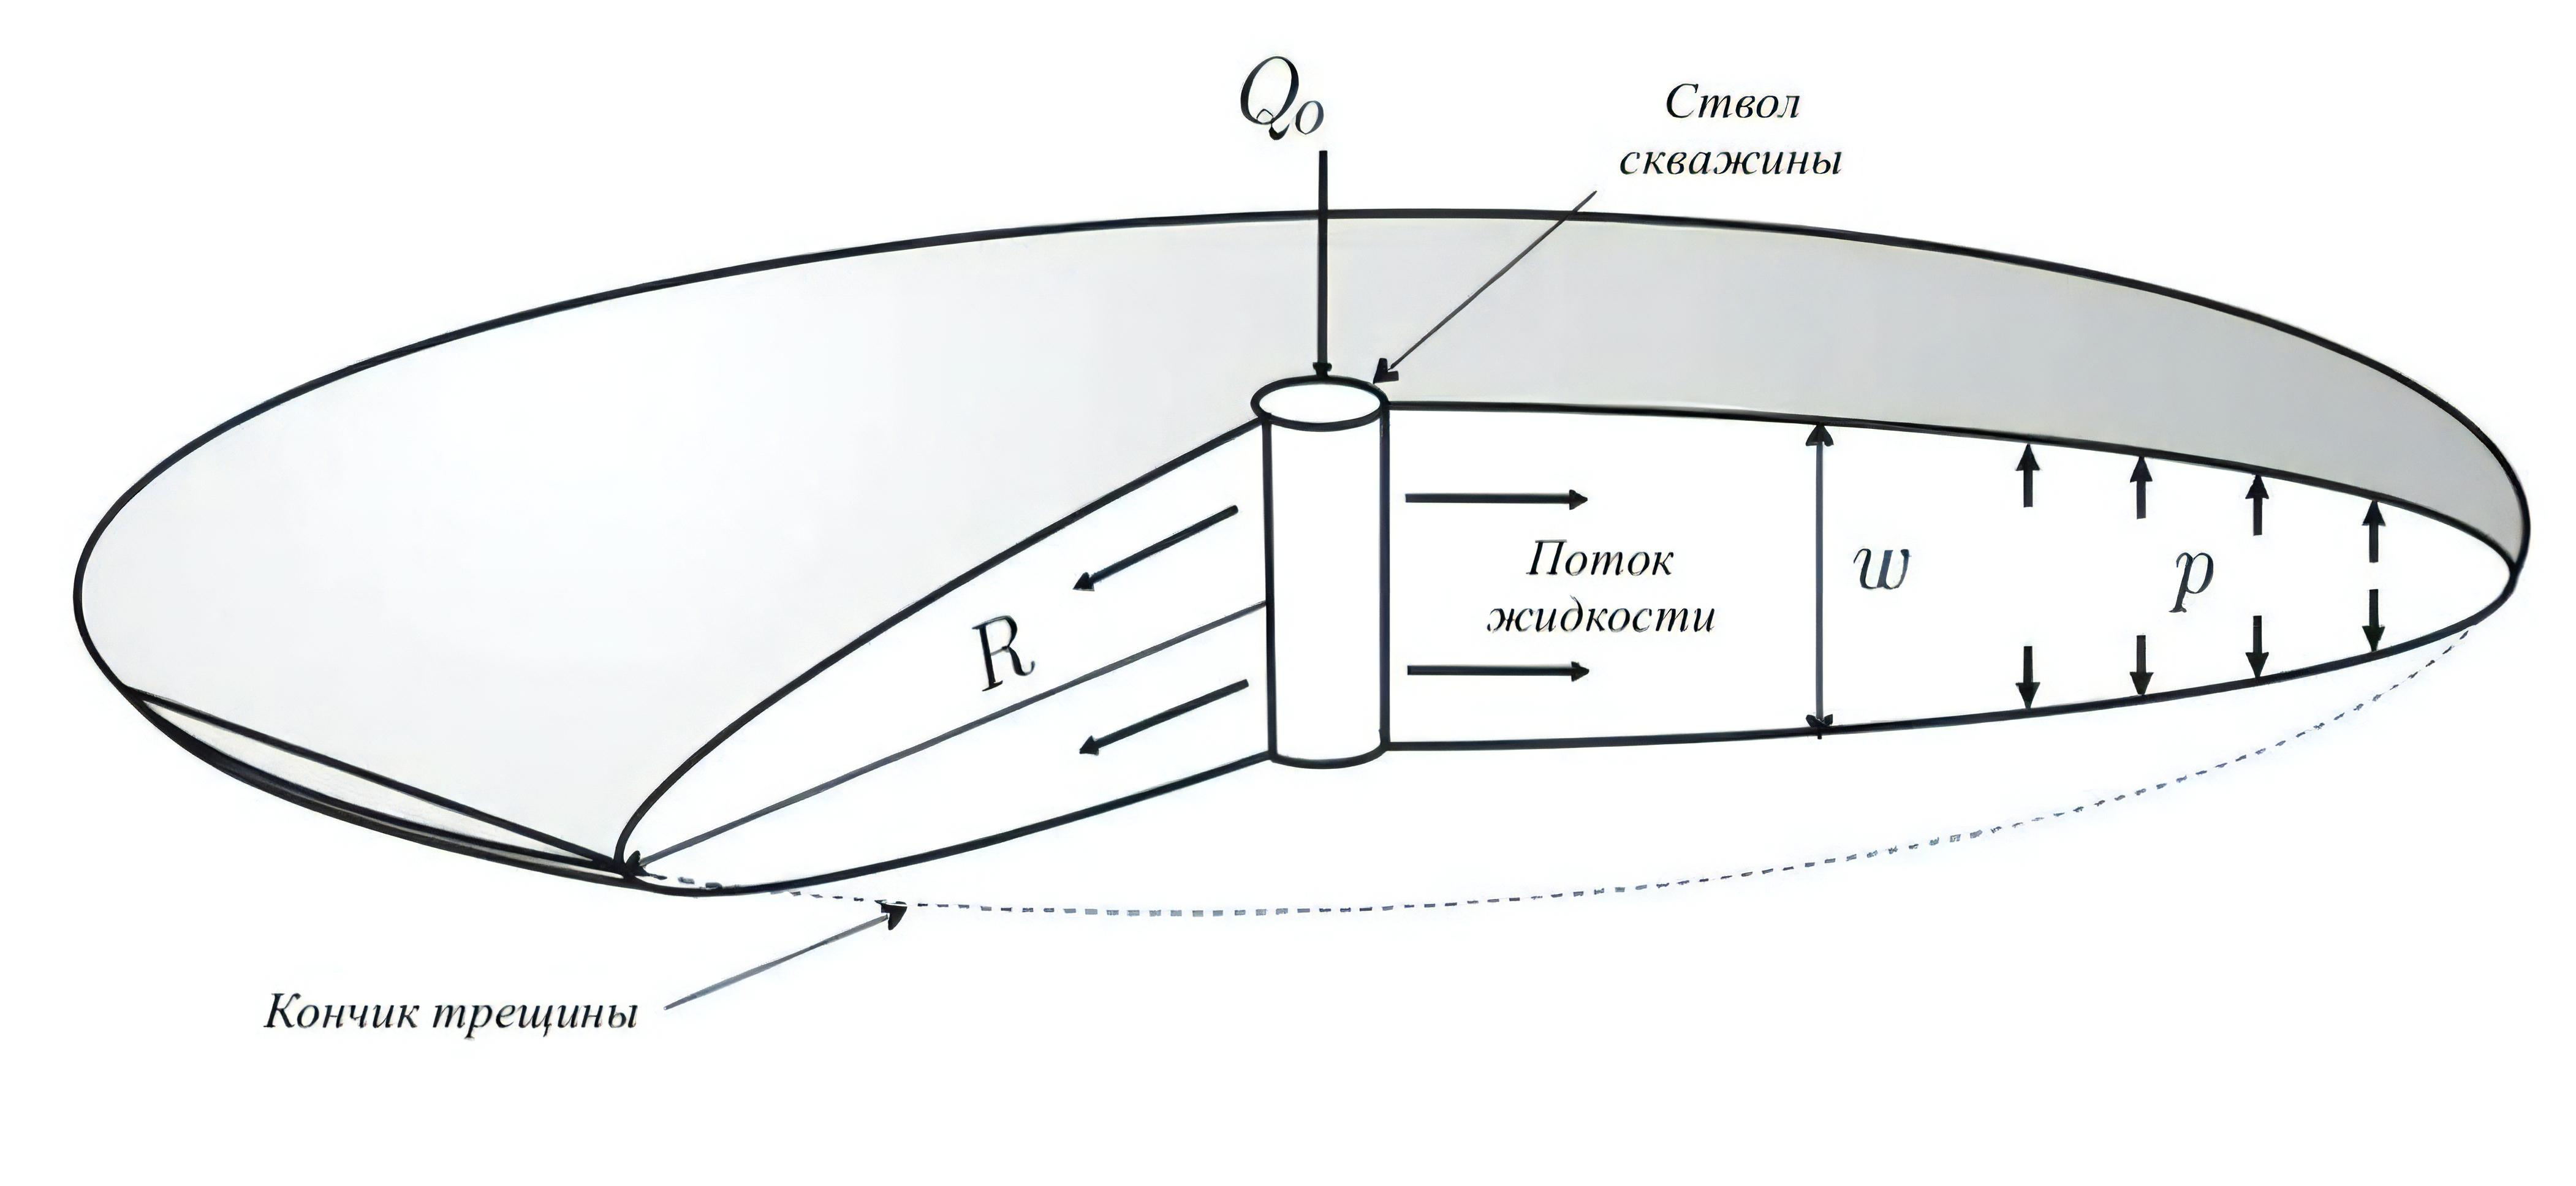
\includegraphics[width=0.7\linewidth]{images/radial_model_better.jpg}
\caption{Геометрия радиальной трещины} 
\label{fig:radial-model-geometry}  
\end{figure}

Система уравнений модели радиальной трещины запишется в следующем виде:
\beq
\begin{cases}
\dfrac{\partial w}{\partial t}+\dfrac{1}{r}\dfrac{\partial}{\partial r}\left(rq\right)+\dfrac{C'}{\sqrt{t-t_0(r)}}=Q_0\delta(r),\\[15pt]
q=-\dfrac{w^3}{\mu'}\dfrac{\partial p_n}{\partial r},\\[5pt]
p_n(r,t)=-\dfrac{E'}{2\pi R}\displaystyle\int\limits_{0}^{R}M\left(\dfrac{r}{R},\dfrac{r'}{R}\right)\dfrac{\partial w(r',t)}{\partial r'}dr',\\[20pt]
\displaystyle\lim_{r\to R}\dfrac{w}{(R-r)^{1/2}}=\dfrac{K'}{E'},
\end{cases}
\eeq
где $C'=2C_l$, $\,\,\,\mu'=12\mu$, $\,\,\,E'=\dfrac{E}{1-\nu^2}$, $\,\,\,K'=\dfrac{8K_{Ic}}{\sqrt{2\pi}}$.
\\

Приближённые решения для модели радиальной трещины представлены в работе \cite{dontsov2}.
Рассмотрены несколько случаев, а именно случай доминирования вязкости с доминированием утечек, случай доминирования вязкости с отсутствием утечек, случай доминирования трещиностойкости с доминированием утечек и случай доминирования трещиностойкости с отсутствием утечек.

\section{Модель Перкинса-Керна-Нордгрена}

\begin{figure}[H]
	\adjustbox{minipage=1.3em,valign=t}{\subcaption{}\label{fig:pkn-model-3D}}%
	\begin{subfigure}[t]{\dimexpr.5\linewidth-1.3em\relax}
		\centering
		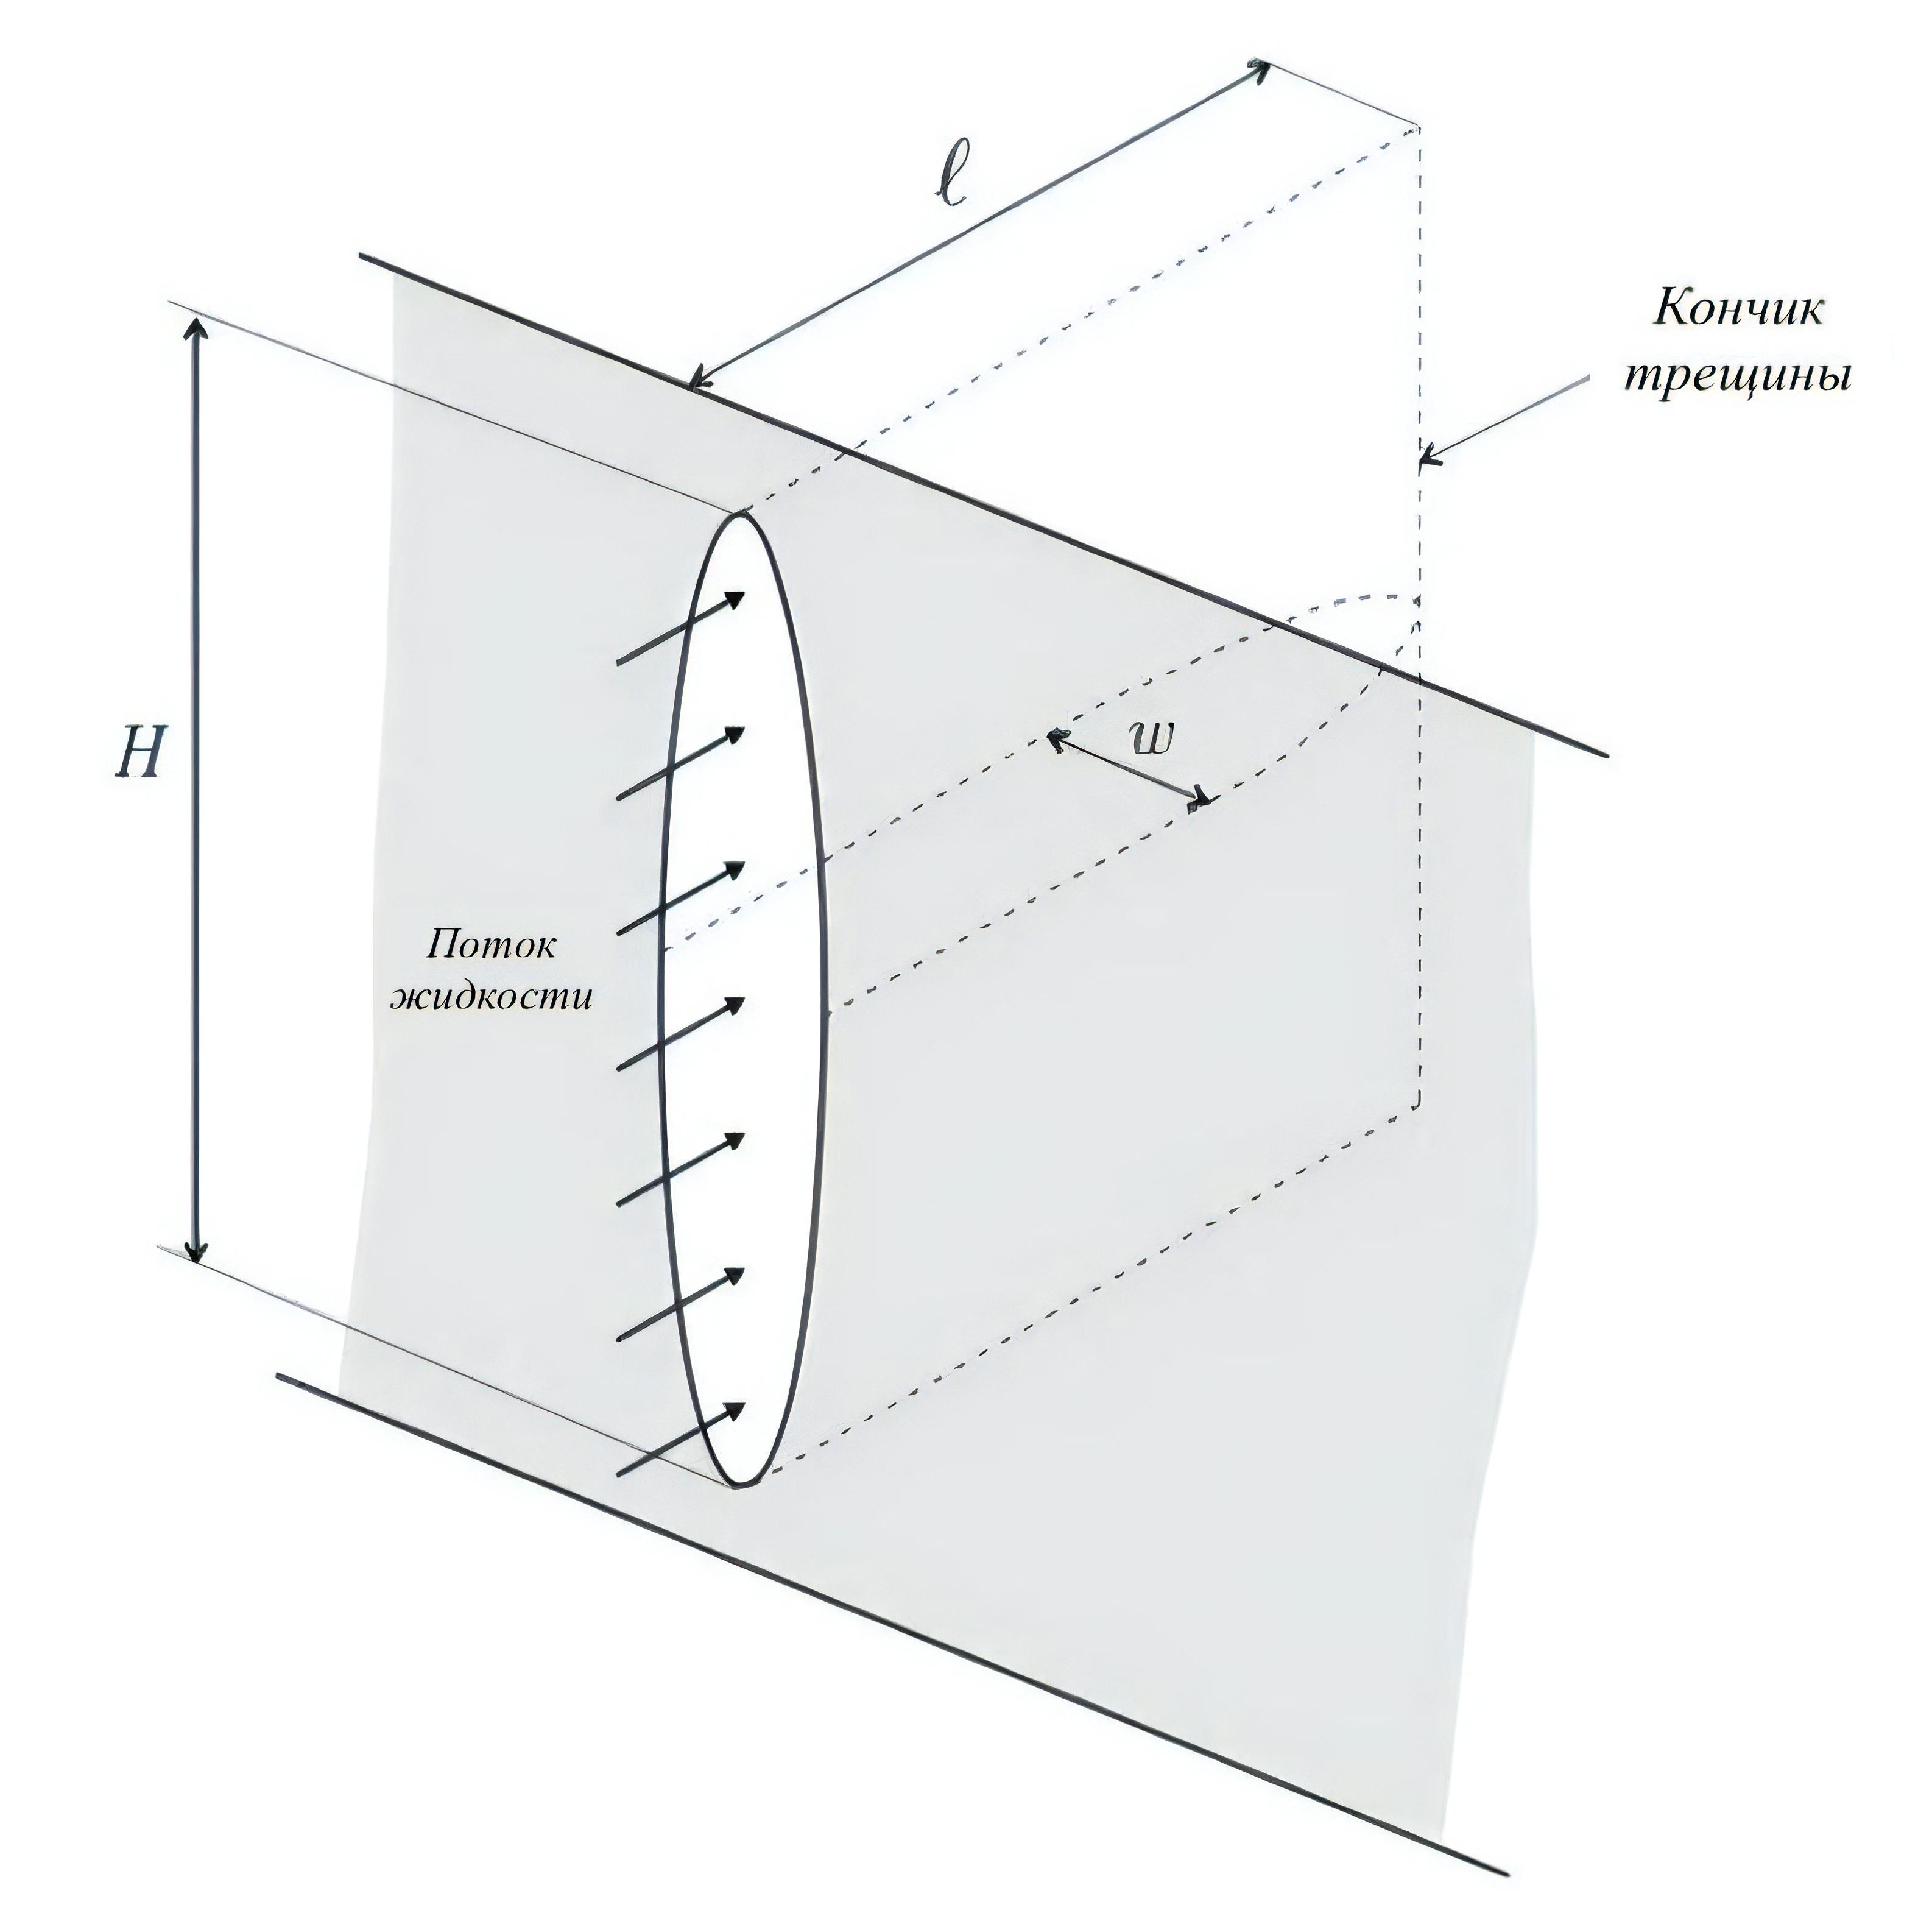
\includegraphics[width=.95\linewidth,valign=t]{images/pkn_model_in_3D_better.jpg}
	\end{subfigure}
\hfill %выровнять по ширине
	\adjustbox{minipage=1.3em,valign=t}{\subcaption{}\label{fig:pkn-model-projections}}%
	\begin{subfigure}[t]{\dimexpr.5\linewidth-1.3em\relax}
		\centering
		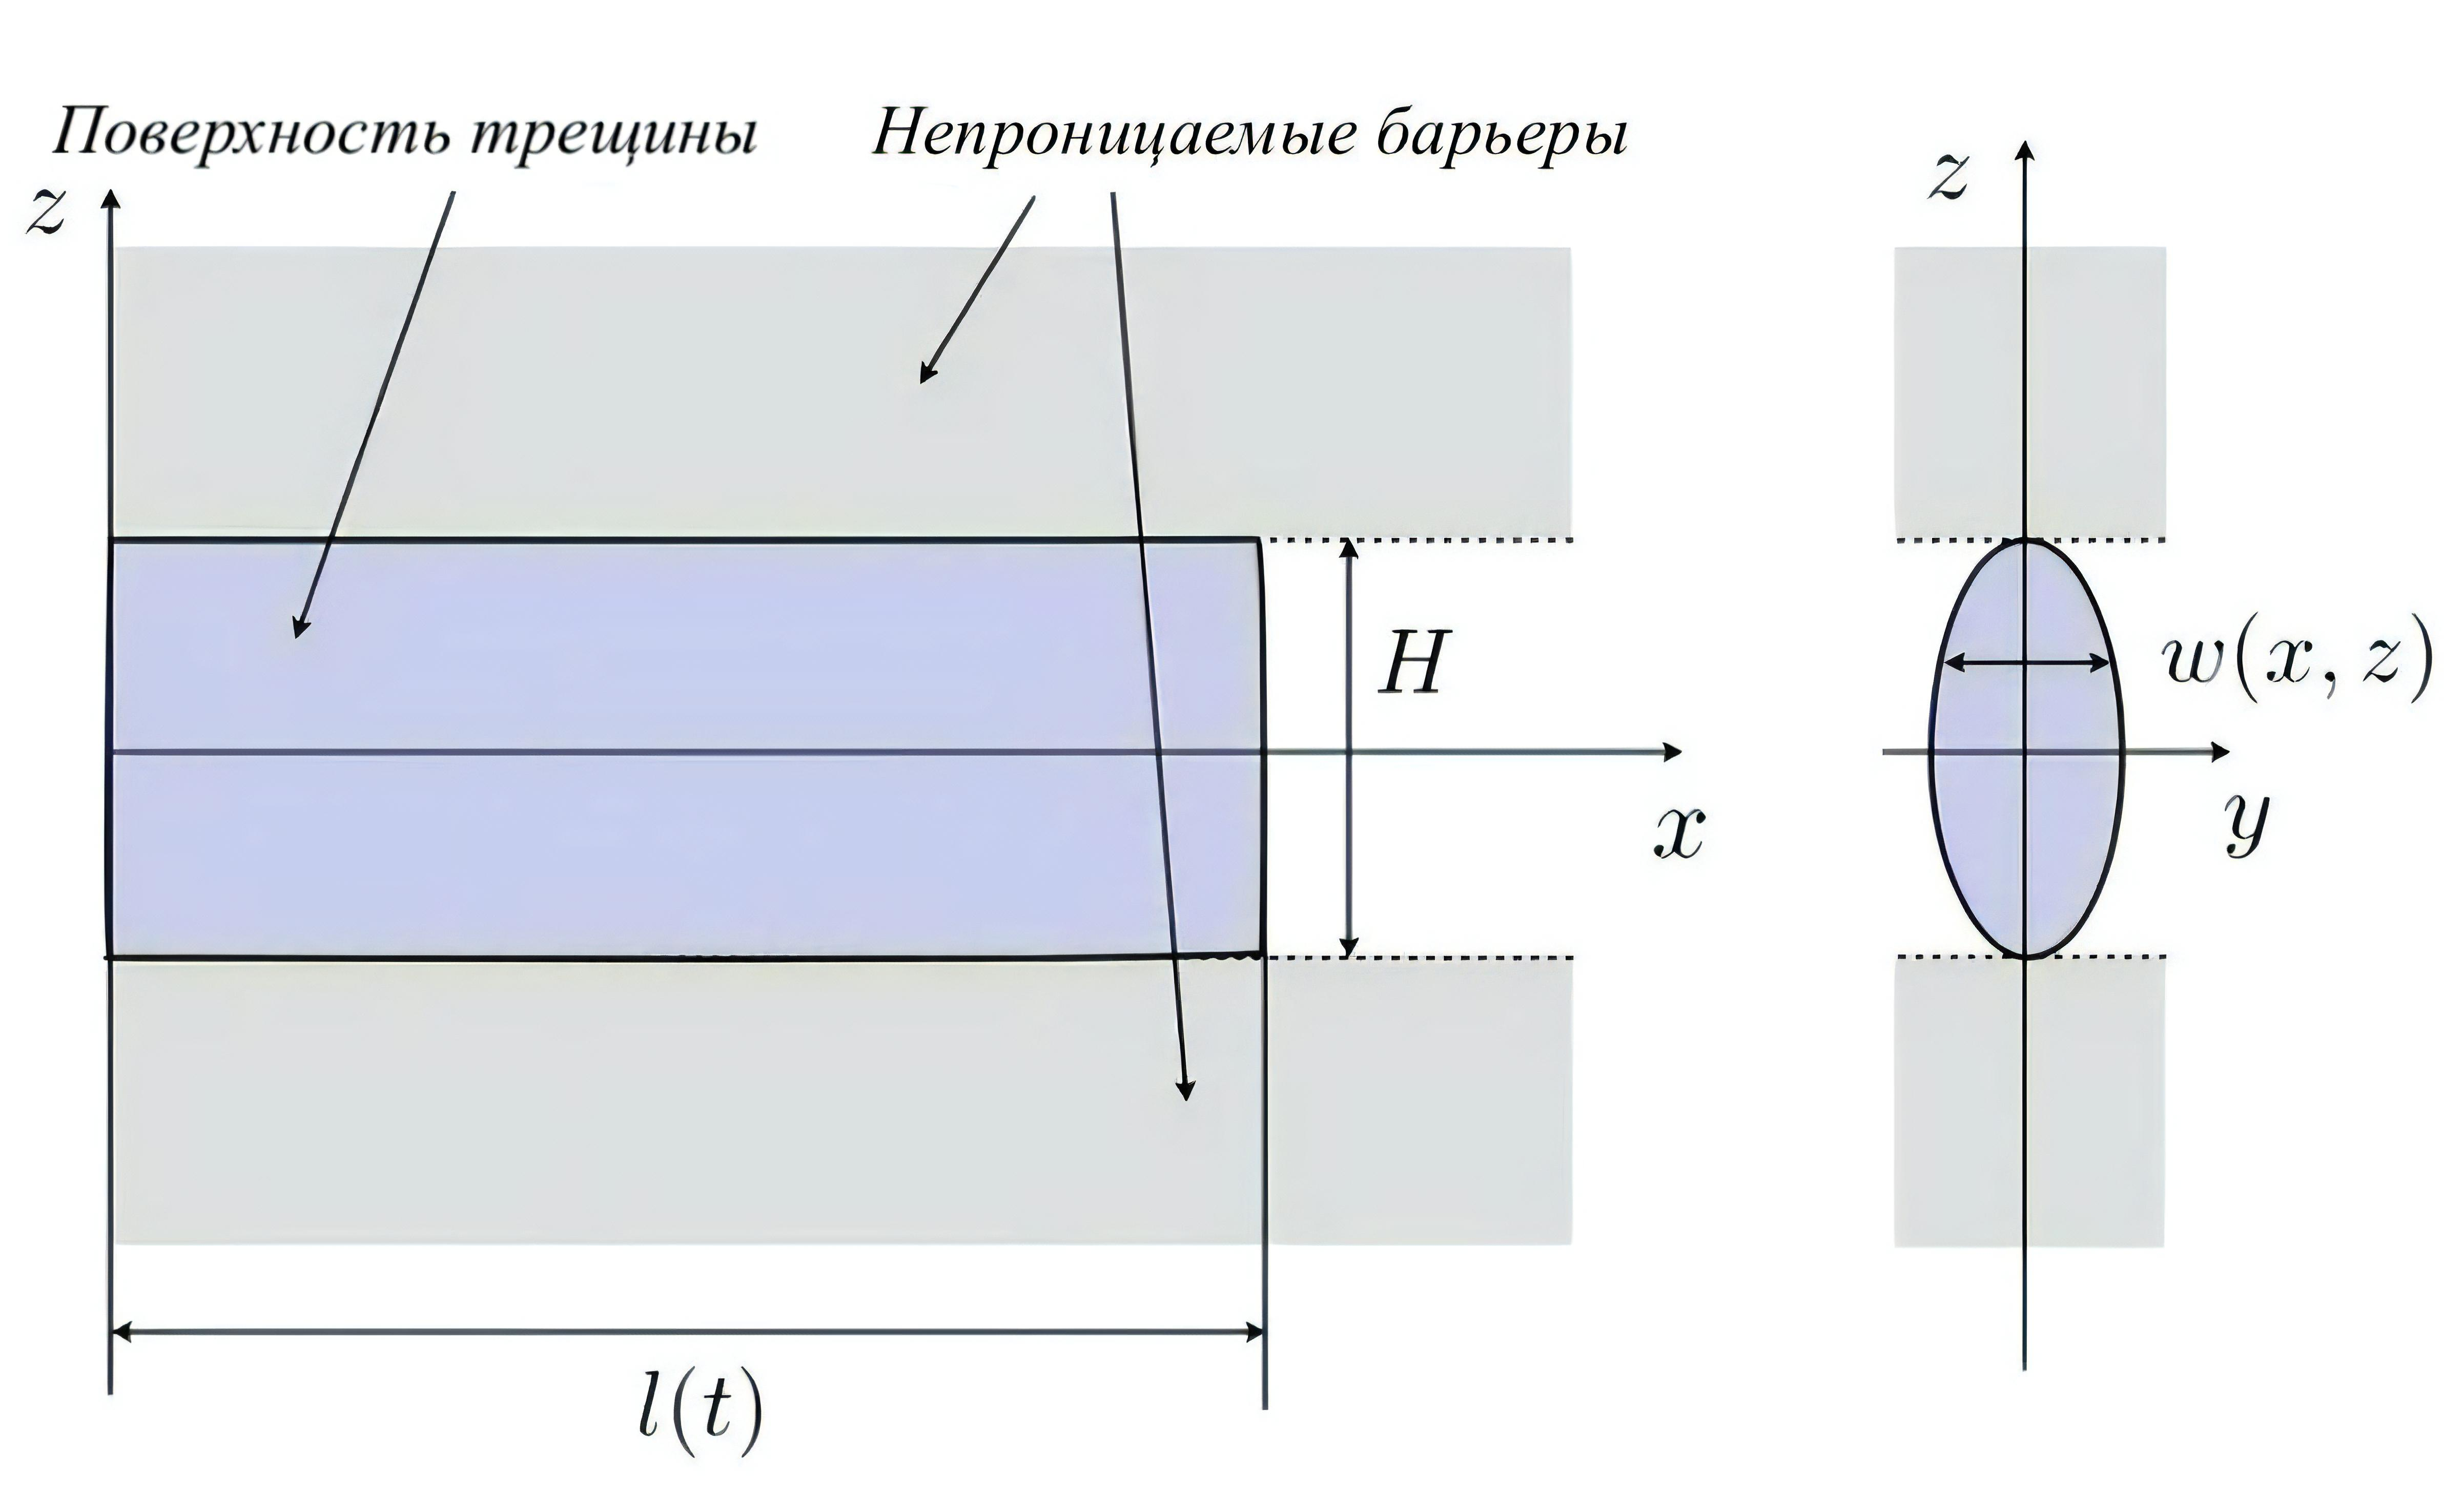
\includegraphics[width=.95\linewidth,valign=t]{images/pkn_model_projections_better.jpg}
	\end{subfigure}
\captionsetup{justification=centering} %центрировать
\caption{Геометрия трещины PKN: {\itshape a} --- в 3D; {\itshape b} --- проекции} 
\label{fig:pkn-model}
\end{figure}

В модели PKN принимается, что условие плоской деформации сохраняется в каждой вертикальной плоскости, нормальной к направлению распространения; однако, в отличие от ситуации строгой плоской деформации, состояние напряжений и деформаций не точно одинаково в следующих одна за другой плоскостях.
Иными словами, в этой модели используется допущение квази-плоской деформации, причём плоскость отсчёта вертикальна и нормальна к направлению распространения.
В модели PKN пренебрегается изменениями давления вдоль вертикальной координаты, а чистое давление $p_{net}$ в трещине рассматривается как функция латеральной координаты $x$.

Система уравнений модели PKN запишется в следующем виде:
\beq
\begin{cases}
\dfrac{\partial\bar{w}}{\partial t}+\dfrac{\partial\bar{q}_x}{\partial x}+\dfrac{C'}{\sqrt{t-t_0(x)}}=\dfrac{Q_0}{H}\delta(x),\\[15pt]
\bar{q}_x=-\dfrac{\bar{w}^3}{\pi^2\mu}\dfrac{\partial p}{\partial x},\\[15pt]
p(x)=-\dfrac{2E'}{\pi^2H}\displaystyle\int\limits_{-l(t)}^{l(t)}\bar{w}(x')\dfrac{dG(2(x'-x)/H)}{dx'}dx',\\[22pt]
\displaystyle\lim_{x\to l}\dfrac{w}{(l-x)^{1/2}}=\dfrac{K'}{E'},
\end{cases}
\eeq
где $C'=2C_l$, $\,\,\,\mu'=12\mu$, $\,\,\,E'=\dfrac{E}{1-\nu^2}$, $\,\,\,K'=\dfrac{8K_{Ic}}{\sqrt{2\pi}}$.
\\

Приближённые решения для модели трещины PKN представлены в работе \cite{dontsov2021analysis}.
Рассмотрены несколько случаев, а именно случай доминирования вязкости с доминированием утечек, случай доминирования вязкости с отсутствием утечек, случай доминирования трещиностойкости с доминированием утечек и случай доминирования трещиностойкости с отсутствием утечек.

В работах \cite{koning, nordgren, perkins_kern} показано, что наиболее точно рост трещин автоГРП описывает модель PKN в случае доминирования трещиностойкости и больших утечек жидкости в пласт.

%\beq
%\frac{\partial\sigma_{xx}}{\partial x}+\frac{\partial\sigma_{xy}}{\partial y}=0
%\eeq


%\section{Название параграфа} \label{ch2:sec1}


